\documentclass[pdflatex,sn-nature]{sn-jnl}

\usepackage{graphicx}
\usepackage{amsmath,amssymb}
\usepackage{xcolor}
\usepackage{textcomp}
\usepackage{url}

\begin{document}

\title[Response to Reviewers]{Response to Reviewers}

\author[1]{\fnm{Xiaoxu} \sur{Shi}}
\author*[2,1]{\fnm{Jiping} \sur{Liu}}\email{liujp63@awi.de}
\author[1]{\fnm{Hu} \sur{Yang}}
\author[1]{\fnm{Chaoyuan} \sur{Yang}}
\author[3]{\fnm{Gerrit} \sur{Lohmann}}

\affil[1]{\orgname{Southern Marine Science and Engineering Guangdong Laboratory (Zhuhai)}, \orgaddress{\city{Zhuhai}, \country{China}}}
\affil[2]{\orgname{School of Atmospheric Sciences, Sun Yat-sen University}, \orgaddress{\city{Zhuhai}, \country{China}}}
\affil[3]{\orgname{Alfred Wegener Institute, Helmholtz Center for Polar and Marine Research}, \orgaddress{\city{Bremerhaven}, \country{Germany}}}

\maketitle

\textbf{Manuscript:} Glacial--interglacial regime shift in Southern Ocean dense water formation

\medskip

\textbf{Dear Editor and Reviewers,}

\medskip

\textbf{Thank you for the care you have taken with this manuscript. The reports are detailed and
constructive, and several of them identify a problem that we had handled too lightly in the
submitted version, namely the disagreement between our pre-industrial result and observation-based
transformation estimates for the modern Southern Ocean. We took that criticism seriously and spent
most of the revision on it. Rather than defend the original one-sentence explanation, we ran the
diagnostic tests that Reviewers 2 and 3 proposed. The outcome is more informative than we expected
and it has changed how we frame the paper.}

\medskip

\textbf{In the following we reproduce every reviewer comment in full and respond to each in turn.
Our replies are written in blue, and new or modified manuscript text is given in blue italics
inside quotation marks. Figures are numbered per reviewer, so Reviewer~1 is referred to
Figs.~R1.1--R1.3, Reviewer~2 to Figs.~R2.1--R2.3 and Reviewer~3 to Figs.~R3.1--R3.6. Where several
reviewers raised the same point the relevant figure is repeated in each section, so that no
reviewer needs to consult another reviewer's response.}

\medskip

\textbf{Thanks again for your time and effort.}

\medskip

\textbf{Best regards,}

\textbf{Xiaoxu Shi, on behalf of all co-authors}

\medskip

\section*{Summary of the main changes}

\textbf{Five new figures and one new table have been added, together with a Source Data file.
The principal changes are:}

\begin{enumerate}
\item \textbf{The disagreement with Pellichero et al. (2018) was tested rather than asserted.} We
recomputed the transformation over their exact domain, the region inside the September 15\% sea ice
contour, which our reproduction matches to within 2.5\% in area. We also converted our density
classes to their neutral density coordinate. The disagreement turns out to be largely a difference
of domain and of density class rather than a wholesale contradiction, and a residual model bias
that we now state plainly.
\item \textbf{The overturning streamfunction and the global ideal age field are now shown
directly}, as Reviewer 3 requested, rather than inferring circulation from ideal age at a single
depth.
\item \textbf{Chen et al. (2025) is now cited and discussed}, with an explicit statement of what
the transformation analysis adds.
\item \textbf{The Southern Annular Mode analysis has been extended} to separate the wind-driven
upwelling from the sea ice salt pump, following Reviewer 3's suggestion.
\item \textbf{A boundary condition table has been added} and all figures now carry climate-state
and coordinate labels.
\end{enumerate}

\clearpage

\section*{Reviewer \#1}

\medskip

The manuscript presents a comprehensive investigation of Southern Ocean dense water formation across a range of glacial and interglacial climates using the AWI-ESM2 Earth system model. By applying a water mass transformation (WMT) framework, the authors successfully separate the relative roles of thermal and haline buoyancy forcing and demonstrate a compelling regime shift between interglacial and glacial climates. The manuscript is well structured, the analyses are technically rigorous, and the decomposition of the different buoyancy contributions provides valuable physical insight. The use of WMT diagnostics allows the underlying mechanisms to be quantified rather than inferred from changes in circulation alone.

Overall, I found the study scientifically interesting and suitable for publication after major revisions. My comments below are primarily intended to strengthen the robustness of the conclusions and improve the clarity of the presentation.

\medskip

\textcolor{blue}{\textbf{We thank the reviewer for this assessment and for the unusually thorough list of
specific comments, which has improved the presentation considerably. We have addressed every point
below.}}

\medskip

\subsection*{General comments}

\medskip

\textbf{Model evaluation and confidence in simulated dense water formation}

\medskip

The conclusions of this study rely entirely on a single Earth system model. While I do not consider this to be a major limitation by itself, I think the manuscript would benefit from a more thorough discussion of how well AWI-ESM2 represents present-day Southern Ocean dense water formation and Antarctic Bottom Water formation. The manuscript briefly states that the PI simulation produces comparable WMT magnitudes to observational estimates, but Figure A4 only shows the model results, making it difficult for the reader to evaluate this statement.

Given the importance of the model for all subsequent paleoclimate interpretations, I encourage the authors to provide stronger evidence supporting its performance. This could include a direct comparison with observational WMT estimates, or a more detailed discussion of known model strengths and biases in Southern Ocean stratification, sea ice, mixed-layer depth, and Antarctic Bottom Water formation. Even if such comparisons already exist in previous AWI-ESM2 publications, briefly summarising them here would substantially increase confidence in the conclusions.

\medskip

\textcolor{blue}{\textbf{We agree, and this concern overlaps with the central criticism from Reviewers 2 and 3.
Our response has three parts.}}

\medskip

\textcolor{blue}{\textbf{First, we now compare the simulated pre-industrial transformation with the
observation-based estimate of Pellichero et al. (2018) over \emph{their} analysis domain rather
than across different domains. Their sector is the region enclosed by the September 15\% sea ice
contour. Reproducing that definition in our model gives an area within 2.5\% of theirs, so the
comparison is like-for-like. Restricting the integration to the ice-covered sector raises the
haline share, as expected, moving the thermal fraction of the dense-class transformation from 69\%
to 61\% and roughly doubling the sea ice contribution at the transformation maximum from 0.86 to
1.84~Sv (Fig.~\ref{fig:r1domain}).}}

\medskip


\begin{figure}[htbp]
\centering
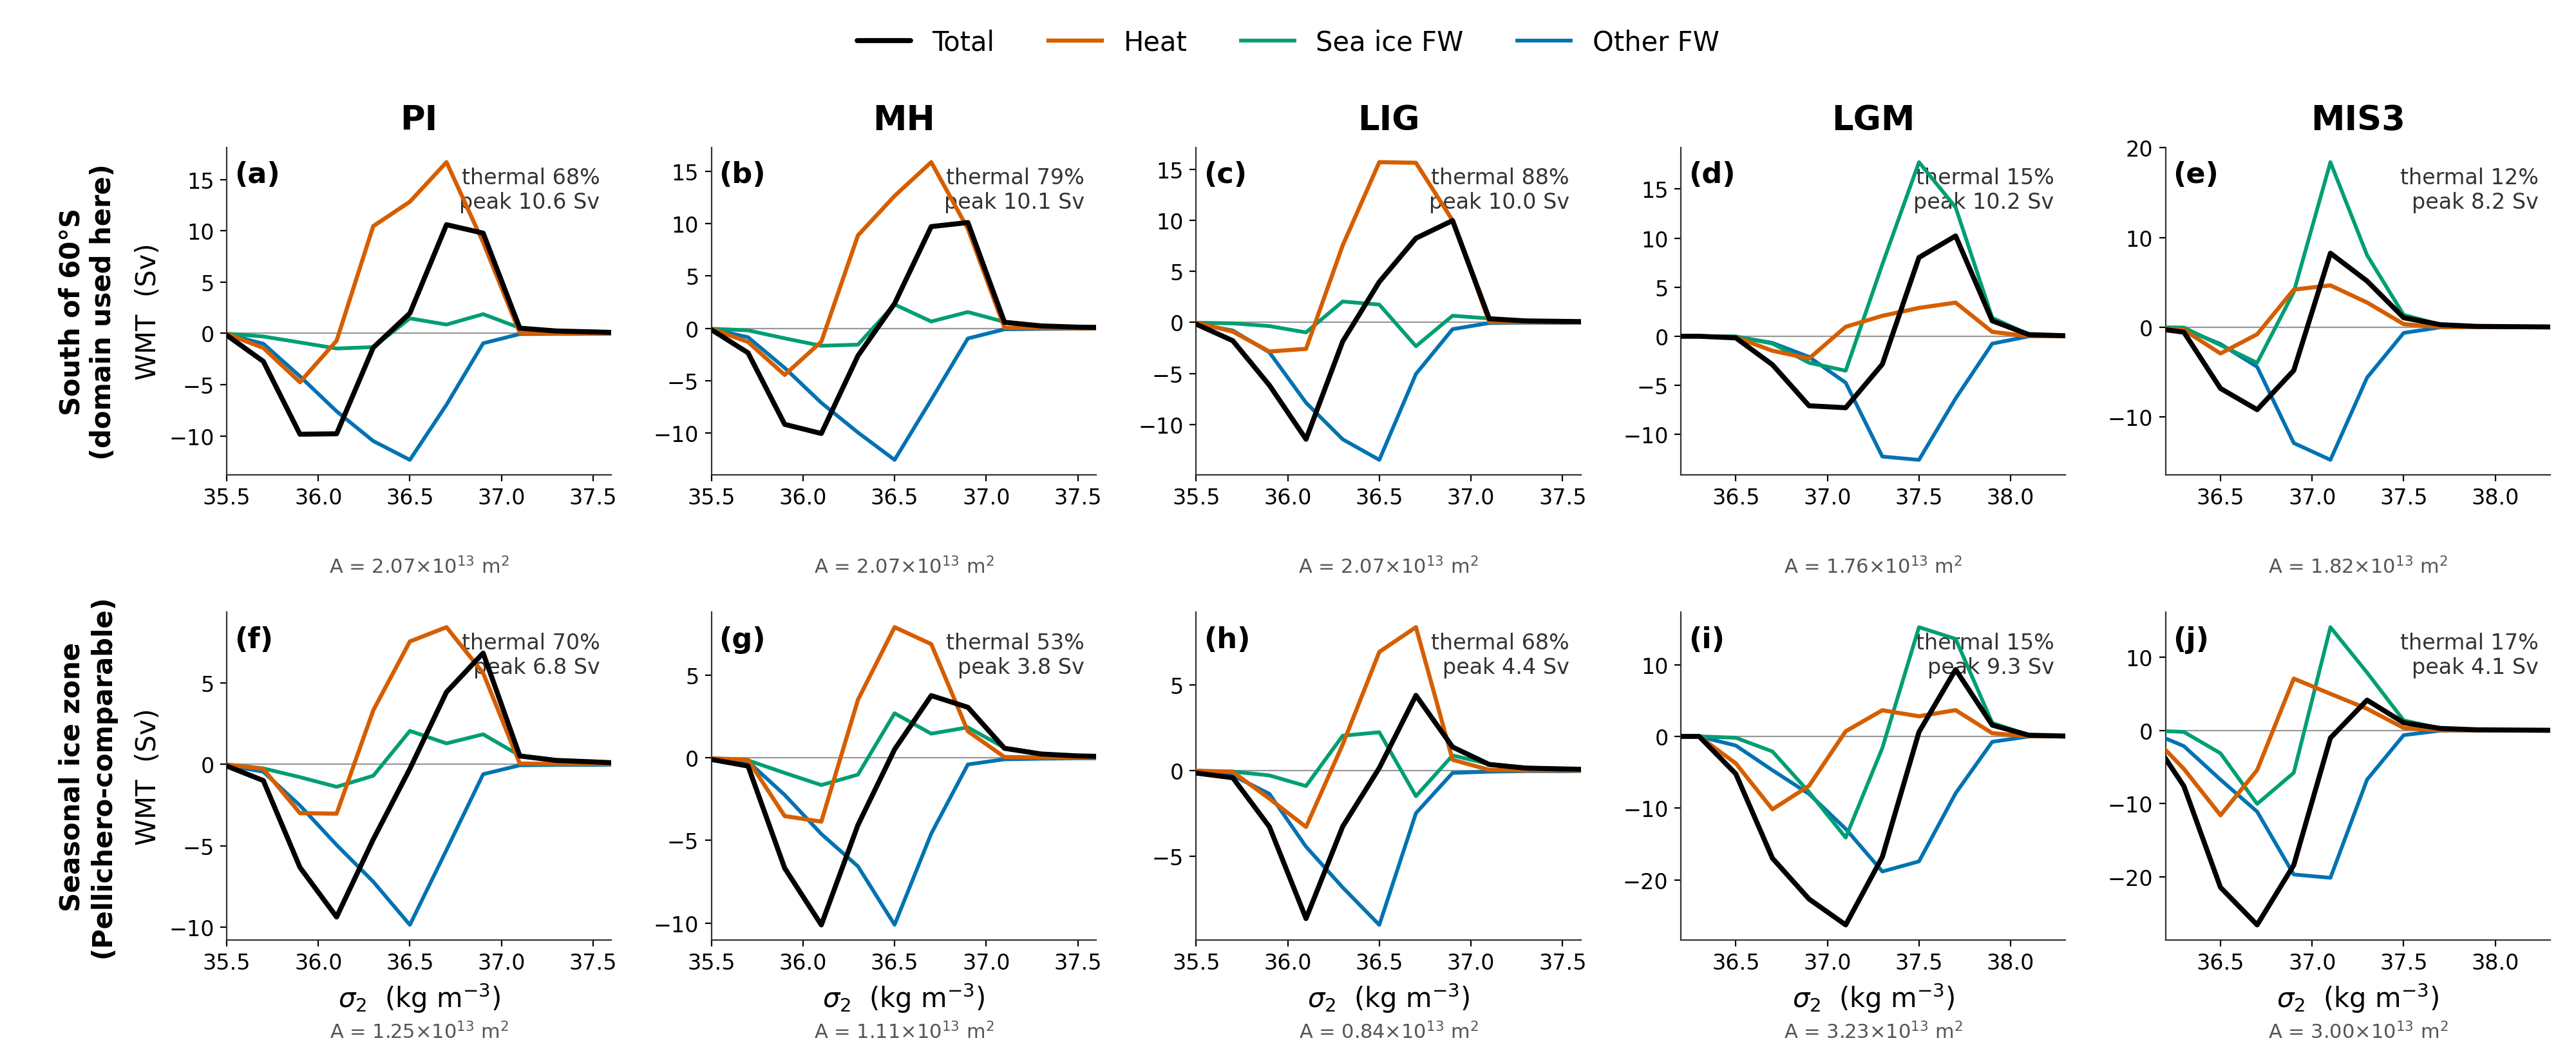
\includegraphics[width=\textwidth]{letter_figs/figR1_wmt_domain_sensitivity.png}
\caption{\textbf{Figure R1.1} (manuscript Fig.~8). Transformation integrated south of
60$^\circ$S, the domain used in the submitted version (top row), and over the seasonal sea ice
zone alone, which reproduces the domain of Pellichero et al. (2018) to within 2.5\% in area
(bottom row). The thermal share at the transformation maximum and the area of each domain are
given in each panel. The haline share increases in the restricted domain, as expected, but the
contrast between thermally dominated interglacials and haline dominated glacials is unchanged.\label{fig:r1domain}}
\end{figure}

\textcolor{blue}{\textbf{Second, and more importantly, the density range matters more than the domain.
Converting our simulated surface properties to the neutral density coordinate used in that study,
our thermally dominated maximum sits near $\gamma_n \approx 27.3$~kg~m$^{-3}$, whereas their
haline-dominated lower cell occupies $\gamma_n = 27.9$--$28.8$~kg~m$^{-3}$. In the densest classes
our surface fluxes do populate ($\sigma_2 \ge 37.0$~kg~m$^{-3}$), our pre-industrial transformation
is already haline dominated, with 0.79~Sv from sea ice against 0.06~Sv from heat. The two analyses
are therefore largely describing different water masses, and where they overlap they agree in
sign.}}

\medskip

\textcolor{blue}{\textbf{Third, we now state the residual model limitation explicitly rather than alluding to
it. We diagnosed directly where the model forms its dense water (Fig.~\ref{fig:r1conv}).}}

\medskip


\begin{figure}[htbp]
\centering
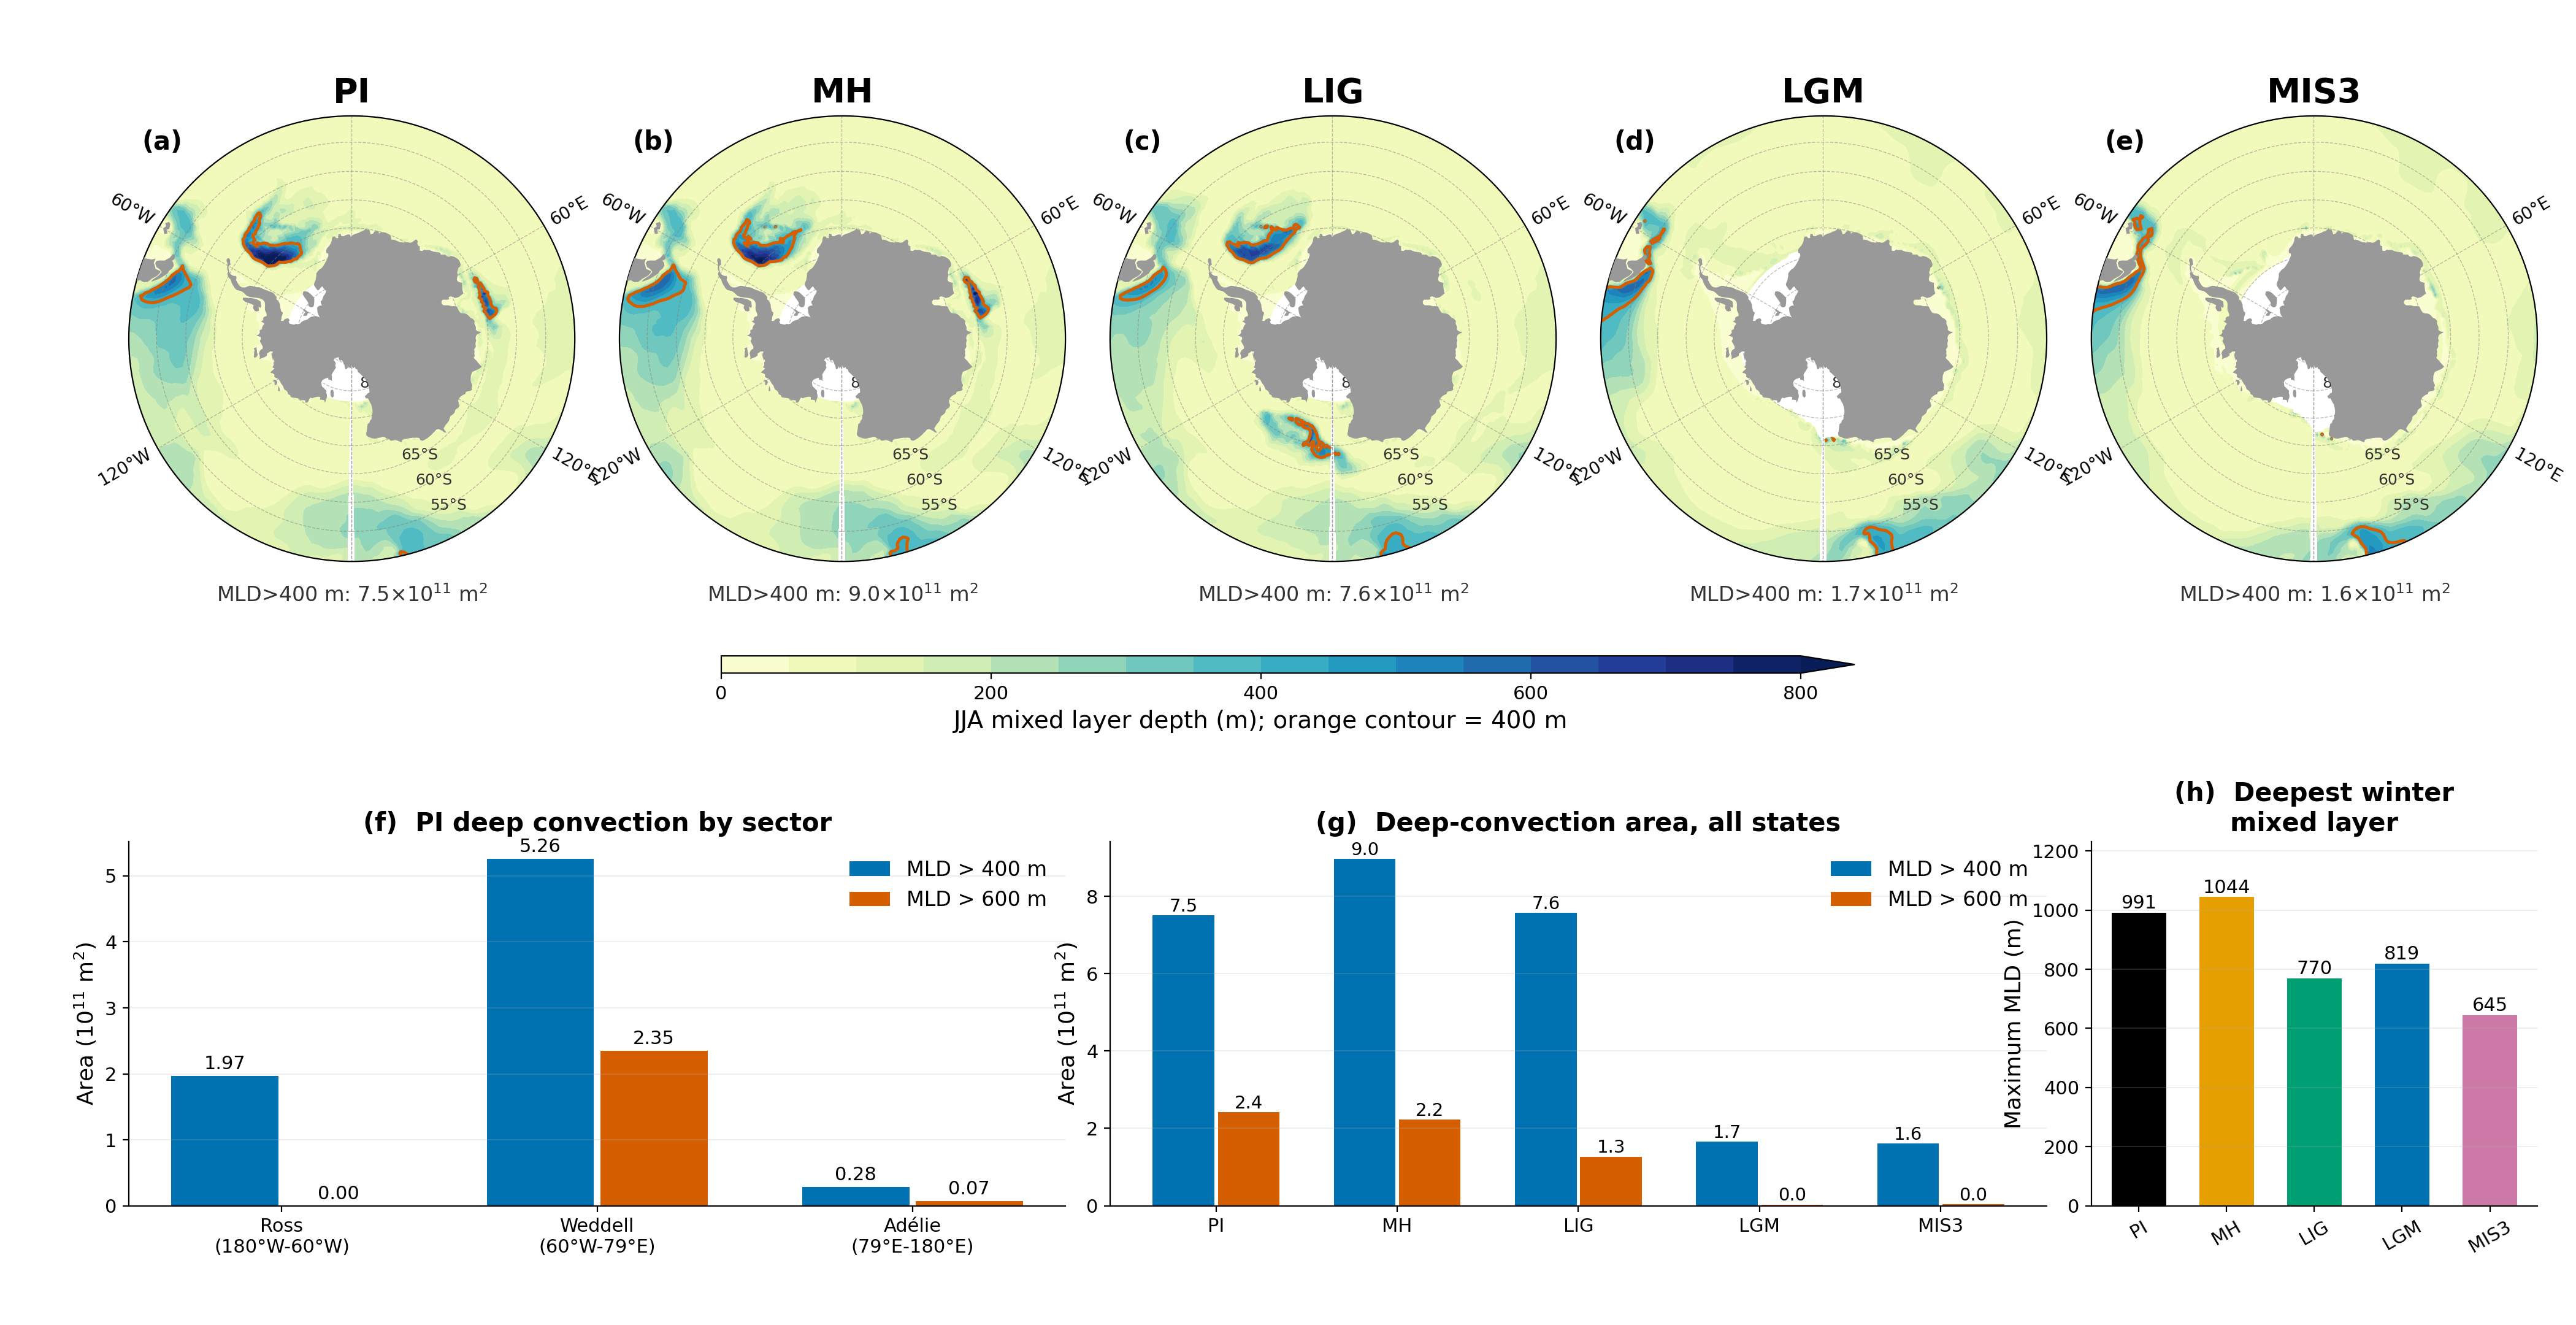
\includegraphics[width=\textwidth]{letter_figs/figR6_convection_sites.png}
\caption{\textbf{Figure R1.2} (new analysis). (a--e) Winter mixed layer depth for the five
states, with the 400~m contour in orange. (f) In the pre-industrial state the Weddell sector
accounts for 70\% of the area with a mixed layer deeper than 400~m and 97\% of the area deeper than
600~m, centred near 68$^\circ$S in the interior of the gyre rather than over the shelf. (g) The
deep-convection area contracts to roughly one fifth of its pre-industrial value in the glacial
states. (h) The deepest winter mixed layer shoals from 991~m in PI to 819~m and 645~m in the
glacials.\label{fig:r1conv}}
\end{figure}

\textcolor{blue}{\textbf{This is open-ocean convection, not the shelf overflow pathway that operates in the
real ocean. We note in the revised Discussion that this is a limitation shared across the current
model generation rather than particular to AWI-ESM2, citing Heuz\'e (2021), who finds that 28 of 35
CMIP6 models form deep and bottom water by open-ocean convection that is too deep, too frequent, or
too extensive, with no model showing convincing shelf export in the Weddell Sea. We also now state
that this configuration has no ice shelf cavities, so basal melt beneath floating ice is absent by
construction.}}

\medskip

\textbf{Boundary conditions}

\medskip

The description of the prescribed boundary conditions for the paleoclimate simulations could be expanded. In particular, the glacial simulations use the GLAC-1D ice-sheet reconstruction, but it is not entirely clear how the ice-sheet changes are implemented in the model (e.g., topography, land-sea mask, ice-sheet extent, bathymetry, or other boundary conditions). As Antarctic dense water formation is highly sensitive to such factors, providing additional details on the experimental setup would help readers assess the robustness of the simulations.

This is not a request for additional simulations, but rather for a clearer discussion of the robustness of the conclusions and the extent to which they may depend on the chosen model configuration and forcing datasets.
A summary table listing the prescribed greenhouse gas concentrations, orbital parameters, and ice-sheet boundary conditions for each experiment would also improve the readability of the Methods section.

\medskip

\textcolor{blue}{\textbf{Added. Table~1 of the revised Methods now lists the greenhouse gas concentrations,
orbital parameters and ice sheet configuration for all five experiments; the values are those
actually used in the runs, read from the model configuration files. We have also expanded the
surrounding text to describe how GLAC-1D enters the model, which we agree was underspecified:}}

\medskip

\textcolor{blue}{\textbf{	extit{``The GLAC-1D reconstruction enters the model through several boundary fields
simultaneously. It sets the ice sheet extent and surface elevation and the associated land-sea mask
and orography used by the atmosphere and land-surface components, the river routing, and the
vegetation distribution. It also determines the ocean bathymetry and coastline, which requires a
dedicated unstructured ocean mesh for each glacial period; we use meshes constructed for 21~ka and
38~ka respectively, while PI, MH and LIG share the modern-geometry mesh. Global mean ocean salinity
is raised in the glacial experiments to account for the water stored in the ice sheets. No
prescribed ice sheet meltwater flux is applied in any of the equilibrium simulations, and the model
configuration does not include ice shelf cavities, so basal melt beneath floating ice shelves is not
represented.''}}}

\medskip

\textbf{Clarifying several interpretations}

\medskip

Most interpretations are convincing, although a few statements could be presented more carefully or supported more explicitly. For example, some descriptions of the role of the Southern Annular Mode appear stronger than the presented evidence suggests, and several discussions would benefit from more direct references to the relevant figure panels.

\medskip

\textcolor{blue}{\textbf{We have moderated the Southern Annular Mode claims. The most overstated passage was
the suggestion that the simulated coupling implies a route to marine proxy reconstruction; we have
replaced it with a more careful statement noting that the accumulation rates and chronological
precision required are rarely available around the Antarctic margin, a point Reviewer 3 also
raised. We have also removed the claim that the circumpolar picture holds uniformly and now state
explicitly where it does not, in particular the Ross Sea. Panel-level figure references have been
added throughout.}}

\medskip

\textbf{Model limitations}

\medskip

Model limitations: The manuscript convincingly demonstrates that sea ice drives the transition from a thermally dominated to a haline-dominated dense water formation regime. However, the discussion would benefit from a brief consideration of the known biases and limitations of AWI-ESM2, particularly regarding Southern Ocean sea ice, mixed-layer depths, and Antarctic Bottom Water formation. Discussing how these model characteristics may influence the proposed mechanism would help readers assess the robustness and broader applicability of the conclusions.

\medskip

\textcolor{blue}{\textbf{Addressed in the Discussion, as described above. We additionally discuss two
limitations that bear on the interpretation. The first is the glacial wind field: our simulated
westerlies shift poleward and strengthen, whereas proxy reconstructions infer an equatorward shift
of about 4.8$^\circ$ and a weakening of about 25\% at the Last Glacial Maximum relative to the
mid-Holocene (Gray et al., 2023). The second is that the ideal age fields are not fully equilibrated
after 1000 years, so the simulated ages are lower bounds. Both are now stated in the text.}}

\medskip

\textbf{Figure labelling and subpanel references}

\medskip

Please consider adding latitude and longitude labels to all map figures where appropriate. In addition, referring to specific figure subpanels throughout the text, rather than only the full figure number, would make the discussion easier to follow.

\medskip

\textcolor{blue}{\textbf{Subpanel references have been added throughout the Results and Discussion. The polar
stereographic panels now carry labelled latitude circles, and the ventilation age maps carry
labelled meridians as well. On the fifteen-panel composite figures we label the latitude circles
only, because a full graticule with meridian labels on panels of that size was illegible in trial
versions. We are happy to add complete labelling if the reviewer prefers.}}

\medskip

\subsection*{Specific comments}

\medskip

1. ' LIG, LGM and MIS should be capitalised.

\medskip

\textcolor{blue}{\textbf{Corrected throughout.}}

\medskip

2. Line 21-22: The transition to SAM is quite abrupt.

\medskip

\textcolor{blue}{\textbf{The abstract now introduces the Southern Annular Mode through the mechanism that connects it
to the mean state In the revised manuscript this now reads: \textit{``Because the balance between these two pathways is set by how much of the surface is ice covered, it also governs the response to internal atmospheric variability. The Southern Annular Mode modulates transformation by 3-8 Sv between its positive and negative phases in every climate state, working through heat loss when the ocean is open and through brine rejection when it is ice covered.''}, noting that because the balance between the thermal and haline pathways is set
by how much of the surface is ice covered, it also governs the response to internal atmospheric
variability.}}

\medskip

3. Line 24: "same mechanisms" sounds vague her without additional context. The abstract should be understandable on its own without requiring the reader to refer to the main text.

\medskip

\textcolor{blue}{\textbf{Replaced with an explicit statement. The abstract now reads that the mode works ``through heat
loss when the ocean is open and through brine rejection when it is ice covered''.}}

\medskip

4. Lines 25-27: Similar to Comment 2 above, additional context is needed before introducing the deep ocean ventilation results. The motivation for analysing ventilation ages only becomes clear later in the manuscript, whereas the abstract should be self-contained.

\medskip

\textcolor{blue}{\textbf{The abstract now bridges from surface forcing to ventilation via the overturning circulation,
stating that weaker glacial transformation coincides with a collapse of the simulated abyssal cell
from about 10 to 2~Sv, before the ages are given. This also incorporates the new overturning
analysis requested by Reviewer 3. In the revised manuscript this now reads: \textit{``Weaker glacial transformation coincides with a collapse of the simulated abyssal overturning cell from about 10 to 2 Sv and with older abyssal water. Ideal ages at 4000 m remain below 500 years during interglacials but exceed 750 years basin-wide during glacials, reaching 1500 years in the Pacific.''}}}

\medskip

5. Lines 102-105: SAM is introduced only briefly here. Given its importance throughout the Results and Discussion, please consider providing a slightly more detailed introduction.

\medskip

\textcolor{blue}{\textbf{The introduction now defines the mode as the leading mode of extratropical Southern Hemisphere
variability, describes what its positive phase does to the westerlies and hence to Ekman divergence,
air-sea heat exchange and sea ice export, and cites the observational literature linking it to
bottom water changes. In the revised manuscript this now reads: \textit{``The Southern Annular Mode is the leading mode of extratropical Southern Hemisphere circulation variability, describing a meridional redistribution of atmospheric mass between mid-latitudes and Antarctica . Its positive phase strengthens the circumpolar westerlies and displaces them poleward, which changes Ekman divergence, air-sea heat exchange, and the northward export of sea ice. In the present-day ocean these adjustments modulate mixed-layer depth and surface buoyancy forcing , and they have been linked to observed changes in bottom water properties . Whether the mode remains an effective modulator of dense water formation once the mean state changes, in particular once an expanded ice cover separates the ocean from the atmosphere, is not known.''}}}

\medskip

6. Line 125: typo: 'more'

\medskip

\textcolor{blue}{\textbf{Corrected (``moer'' to ``more'').}}

\medskip

7. Line 127: Figure numbering; A3 can't be called before A1 and A2.

\medskip

\textcolor{blue}{\textbf{The appendix figures have been reordered so that they are cited in numerical order.}}

\medskip

8. Line 129: 'Here,'

\medskip

\textcolor{blue}{\textbf{Corrected.}}

\medskip

9. Line 140: As a result, the deep MLD signals, characteristic of open-ocean convection, largely.... Also, "vanish" is perhaps not the most scientific wording.

\medskip

\textcolor{blue}{\textbf{Rephrased to ``are strongly reduced and become confined to narrow coastal bands and
polynyas'', and we now quantify the reduction rather than describing it qualitatively. In the revised manuscript this now reads: \textit{``The reduction is substantial rather than complete. Summed south of 55$^\circ$S, the area with a winter mixed layer deeper than 400 m falls from 7.510$^{11}$ m$^{2}$ in PI to 1.710$^{11}$ m$^{2}$ in LGM and 1.610$^{11}$ m$^{2}$ in MIS3, and the maximum mixed-layer depth decreases from 991 m to 819 m and 645 m. Mixed layers deeper than 600 m, which cover 2.410$^{11}$ m$^{2}$ in PI, essentially disappear in both glacial states. The residual glacial signals in coastal regions are therefore genuinely shallower than their interglacial counterparts, consistent with dense water production that is confined to narrow coastal bands rather than distributed across the open gyres.''}}}

\medskip

10. Line 141: These signals are not particularly visible even in the coastal regions (the darker blue shading in LGM is at ~200m, so considerably shallower than the interglacials).

\medskip

\textcolor{blue}{\textbf{This is a fair objection and we have addressed it with numbers. Summed south of 55$^\circ$S,
the area with a winter mixed layer deeper than 400~m falls from $7.5\times10^{11}$~m$^2$ in PI to
$1.7\times10^{11}$~m$^2$ in LGM and $1.6\times10^{11}$~m$^2$ in MIS3, the maximum mixed-layer depth
decreases from 991~m to 819~m and 645~m, and mixed layers deeper than 600~m essentially disappear
in both glacial states. Panels (g) and (h) of Fig.~\ref{fig:r1conv} make the point quantitatively,
so the reviewer's reading of the shading is correct and is now reflected in the text.}}

\medskip


\begin{figure}[htbp]
\centering
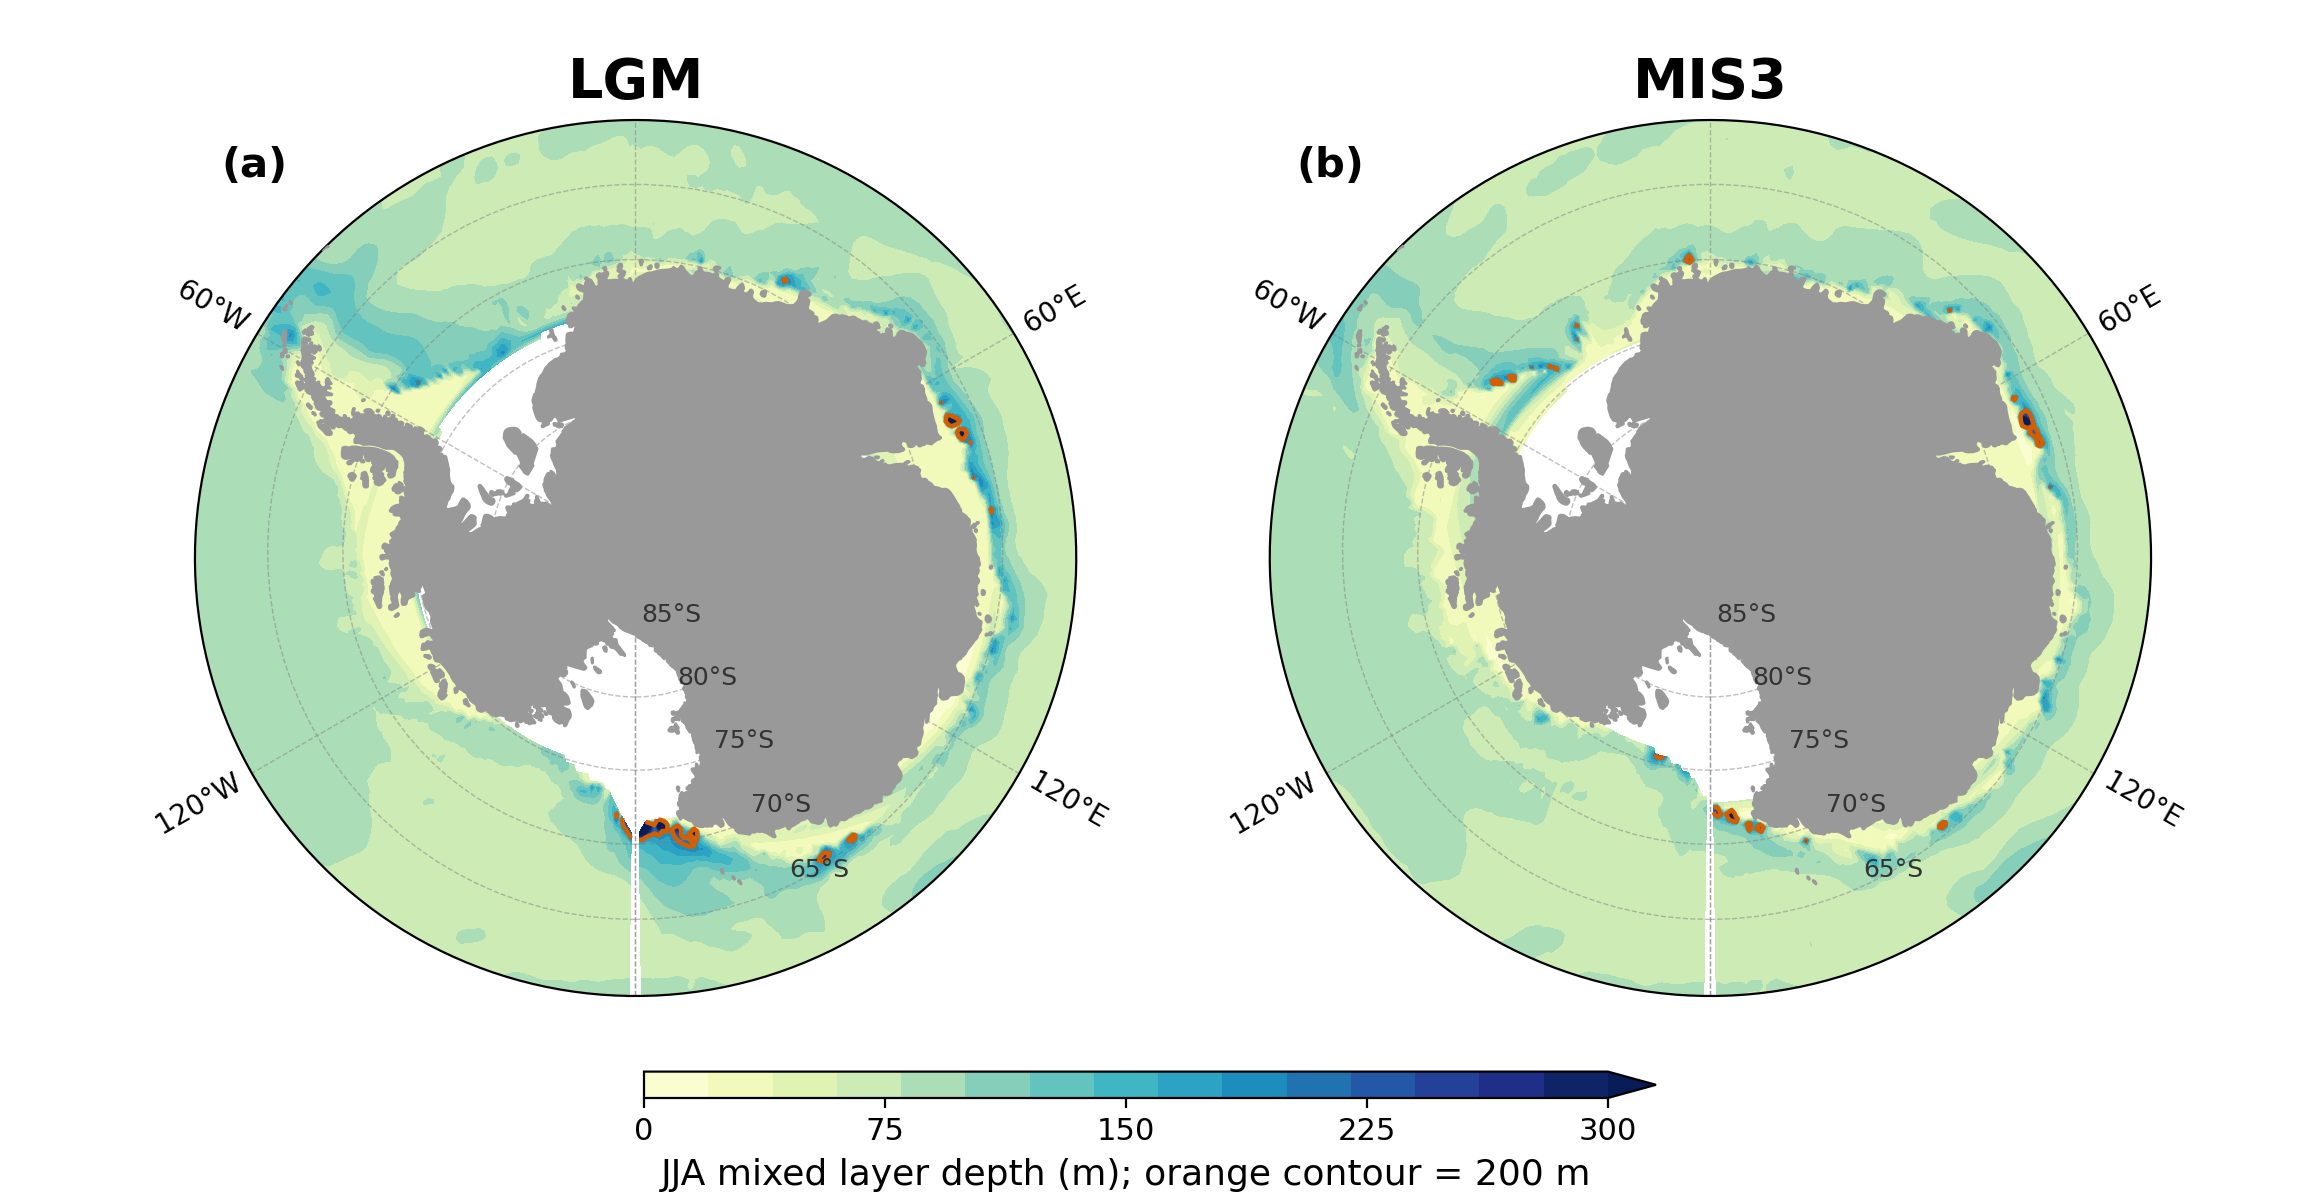
\includegraphics[width=\textwidth]{letter_figs/figR7_mld_glacial_zoom.png}
\caption{\textbf{Figure R1.5} (new supplementary panel). LGM and MIS3 winter mixed
layer depth on the original 0--400~m scale (top) and on a tightened 0--300~m scale with the 200~m
contour marked (bottom). The 99th percentile of the glacial winter mixed layer south of
55$^\circ$S is only 280~m (LGM) and 296~m (MIS3), so the shared interglacial scale leaves the
glacial panels almost featureless. The tightened scale resolves discrete deep cells along the coast,
which is where the glacial dense water is produced.\label{fig:r1mldzoom}}
\end{figure}

11. Line 134-141: Fig.1 i-l subpanels are not discussed at all.

\medskip

\textcolor{blue}{\textbf{A paragraph discussing the surface density panels has been added. It notes that the glacial
density anomalies follow the salinity field rather than the temperature field, because the thermal
expansion coefficient is small at the near-freezing temperatures south of the ice edge, and points
out the density-compensated LIG anomaly and the weak negative LGM anomalies in the
Atlantic--Indian sector. In the revised manuscript this now reads: \textit{``The surface density anomalies (Fig. 1i-l) follow the salinity field rather than the temperature field in the glacial states. Cooling and salinification both act to densify the surface, but at the near-freezing temperatures that prevail south of the ice edge the thermal expansion coefficient is small, so the haline term sets both the pattern and the magnitude. In LIG the warm and salty Bellingshausen-Amundsen anomaly is close to density compensated (Fig. 1j), and the LGM retains weak negative density anomalies in parts of the Atlantic-Indian sector where surface freshening outweighs cooling.''}}}

\medskip

12. Line 144-146: The LIG also exhibits similar behaviour, although the changes are smaller in some basins. Likewise, the LGM shows some negative anomalies in the Atlantic-Indian sector.

\medskip

\textcolor{blue}{\textbf{Both points are now stated in the text, as described in our reply to comment 11.}}

\medskip

13. Line 146-148: An explanation of why the wind stress changes do not lead to increased sea ice in the Ross Sea would be useful. Is this due to the presence of relatively warm water despite enhanced salinity, density, and Ekman transport in this region?

\medskip

\textcolor{blue}{\textbf{We checked this directly, and the answer turned out to be more interesting than the question
assumed. The mechanism the reviewer proposes is real, but it belongs to the last interglacial rather
than to the glacial states the comment refers to. Averaged between 60 and 75$^\circ$S in winter, the
glacial sea ice response is fairly uniform around the continent: concentration rises by 0.62 in the
Ross sector, 0.70 in the Weddell sector and 0.53 in the Ad\'elie sector at the Last Glacial Maximum,
and all three cool to within about 0.1~K of the surface freezing point, so ice growth is not limited
by surface heat content anywhere. The Ross sector separates from the others only in the last
interglacial, where it is 0.97~K warmer than in PI, sits 2.72~K above the freezing point against
changes below 0.3~K elsewhere, and loses 0.19 of its winter ice concentration. There the wind
exports ice efficiently but the water is too far from freezing for it to be replaced, which is
precisely the reviewer's proposed mechanism (Fig.~\ref{fig:r1ross}). We have rewritten the passage
accordingly, rather than attributing the behaviour to the glacial wind response as the submitted
version implied.}}

\medskip


\begin{figure}[htbp]
\centering
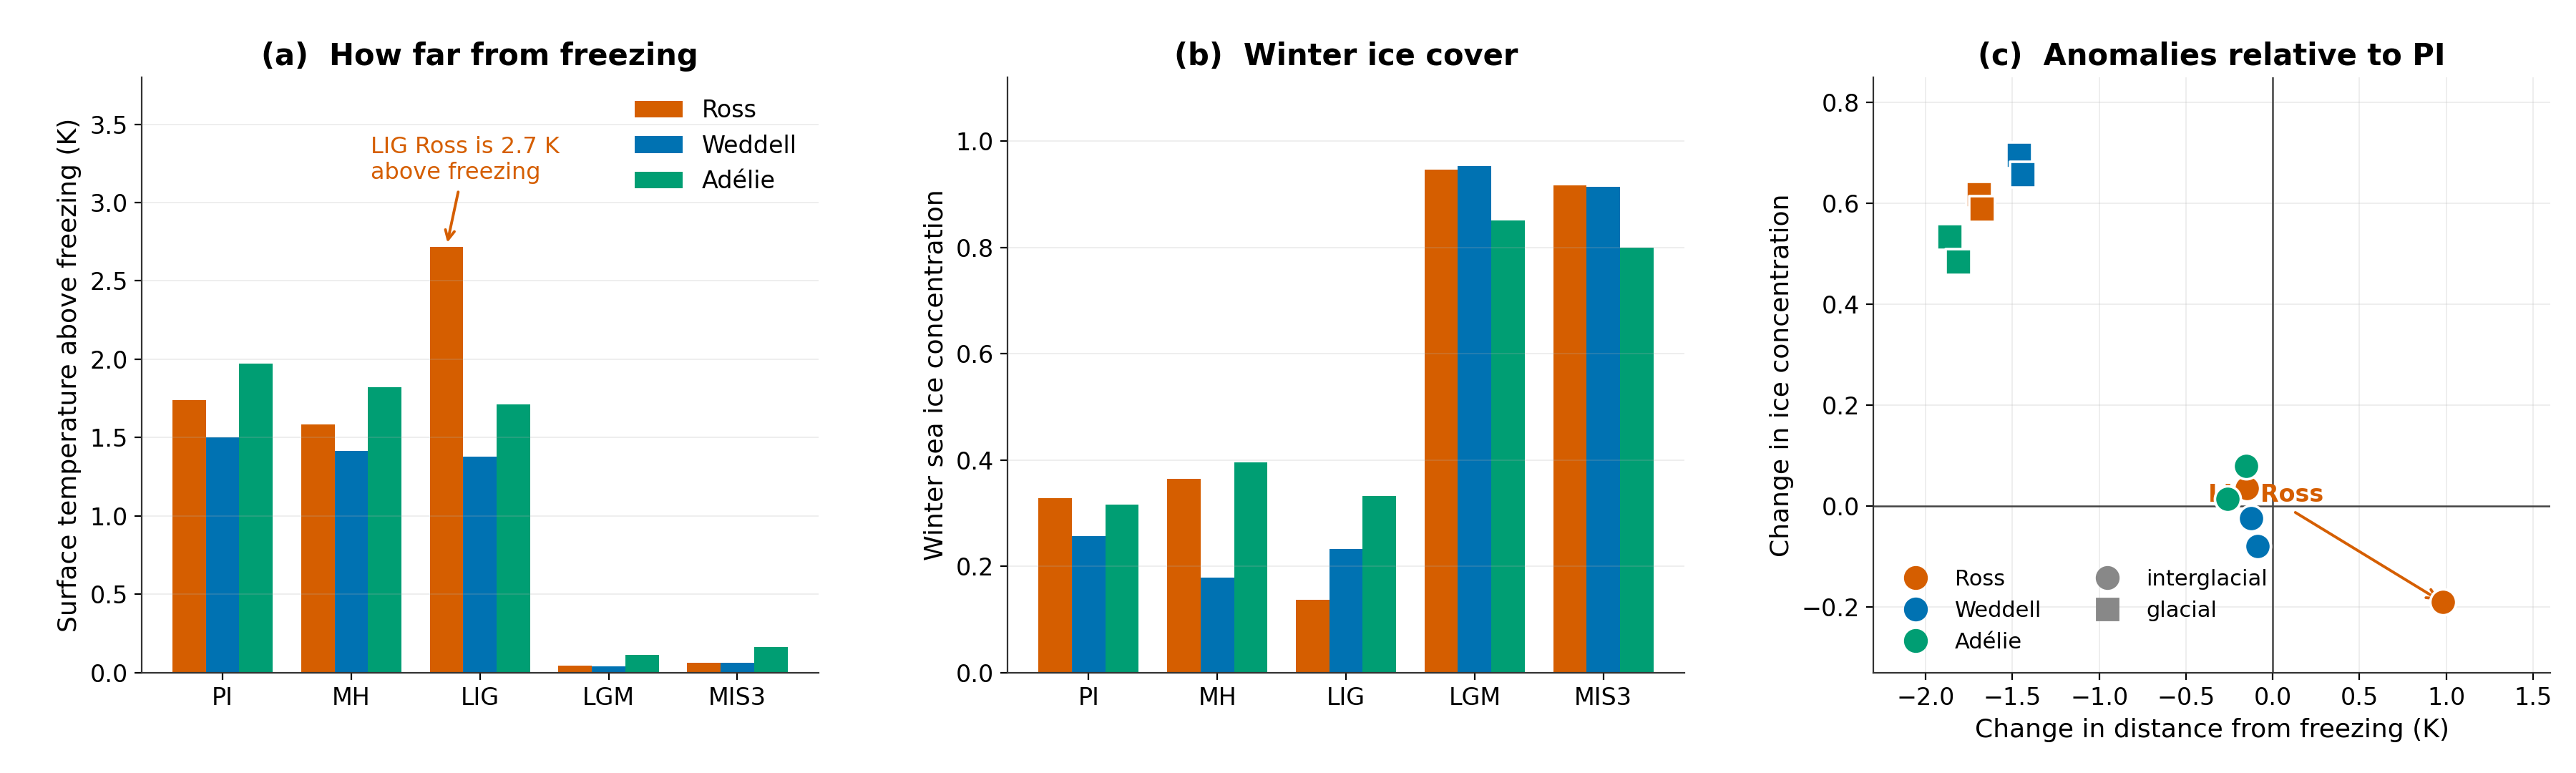
\includegraphics[width=\textwidth]{letter_figs/figR9_ross_sector.png}
\caption{\textbf{Figure R1.4} (new analysis). (a) Winter surface temperature above the
local freezing point and (b) winter sea ice concentration, by sector and climate state. (c) The same
quantities as anomalies relative to PI. The Ross sector separates from the others only in the last
interglacial, where it warms to 2.7~K above freezing and loses 0.19 of ice concentration, an order
of magnitude more than the Weddell or Ad\'elie response. In the glacial states all three sectors
collapse onto the freezing point and gain ice comparably.\label{fig:r1ross}}
\end{figure}

14. Line 167: It would be helpful to quantify the thermal contribution, similar to the quantification provided for the haline contribution in line 157.

\medskip

\textcolor{blue}{\textbf{Added. The thermal term accounts for 70--85\% of the total at the transformation maximum in the
interglacials, against 15--30\% for the haline term, and falls to 12--17\% in the glacial states. In the revised manuscript this now reads: \textit{``This transformation is dominated by surface heat loss (red line), which accounts for 70-85\% of the total at the transformation maximum, with limited sea ice extent restricting the haline contribution from brine rejection to a secondary role (15-30\%; green line). Other freshwater fluxes (blue lines) oppose densification through net precipitation and river runoff. We note that this thermally dominated maximum occurs at densities that correspond to intermediate and mode waters rather than to bottom water. In the densest classes that the simulated surface fluxes reach (\_2 37.0 kg m$^{-3}$), the PI transformation is already haline dominated, with the sea ice term contributing 0.79 Sv against 0.06 Sv from heat in the annual mean. The thermal dominance reported here is therefore a property of the integral over all density classes, and we quantify its sensitivity to the choice of integration domain and density range in the Discussion.''}}}

\medskip

15. Fig. 2 Would it be possible to share a figure with the same y-axis limits for all panels? This may not be necessary for the final manuscript, but it would make it easier to compare the magnitude of the changes across the different climate states.

\medskip

\textcolor{blue}{\textbf{Yes. Supplementary Fig.~S5, reproduced as Fig.~\ref{fig:r1axis} below, shows the same
transformation curves on common vertical and horizontal axes. We have kept the independently scaled
version in the main text because the shape of the individual curves is otherwise hard to read, and
the main text now points to the common-axis version explicitly.}}

\medskip


\begin{figure}[htbp]
\centering
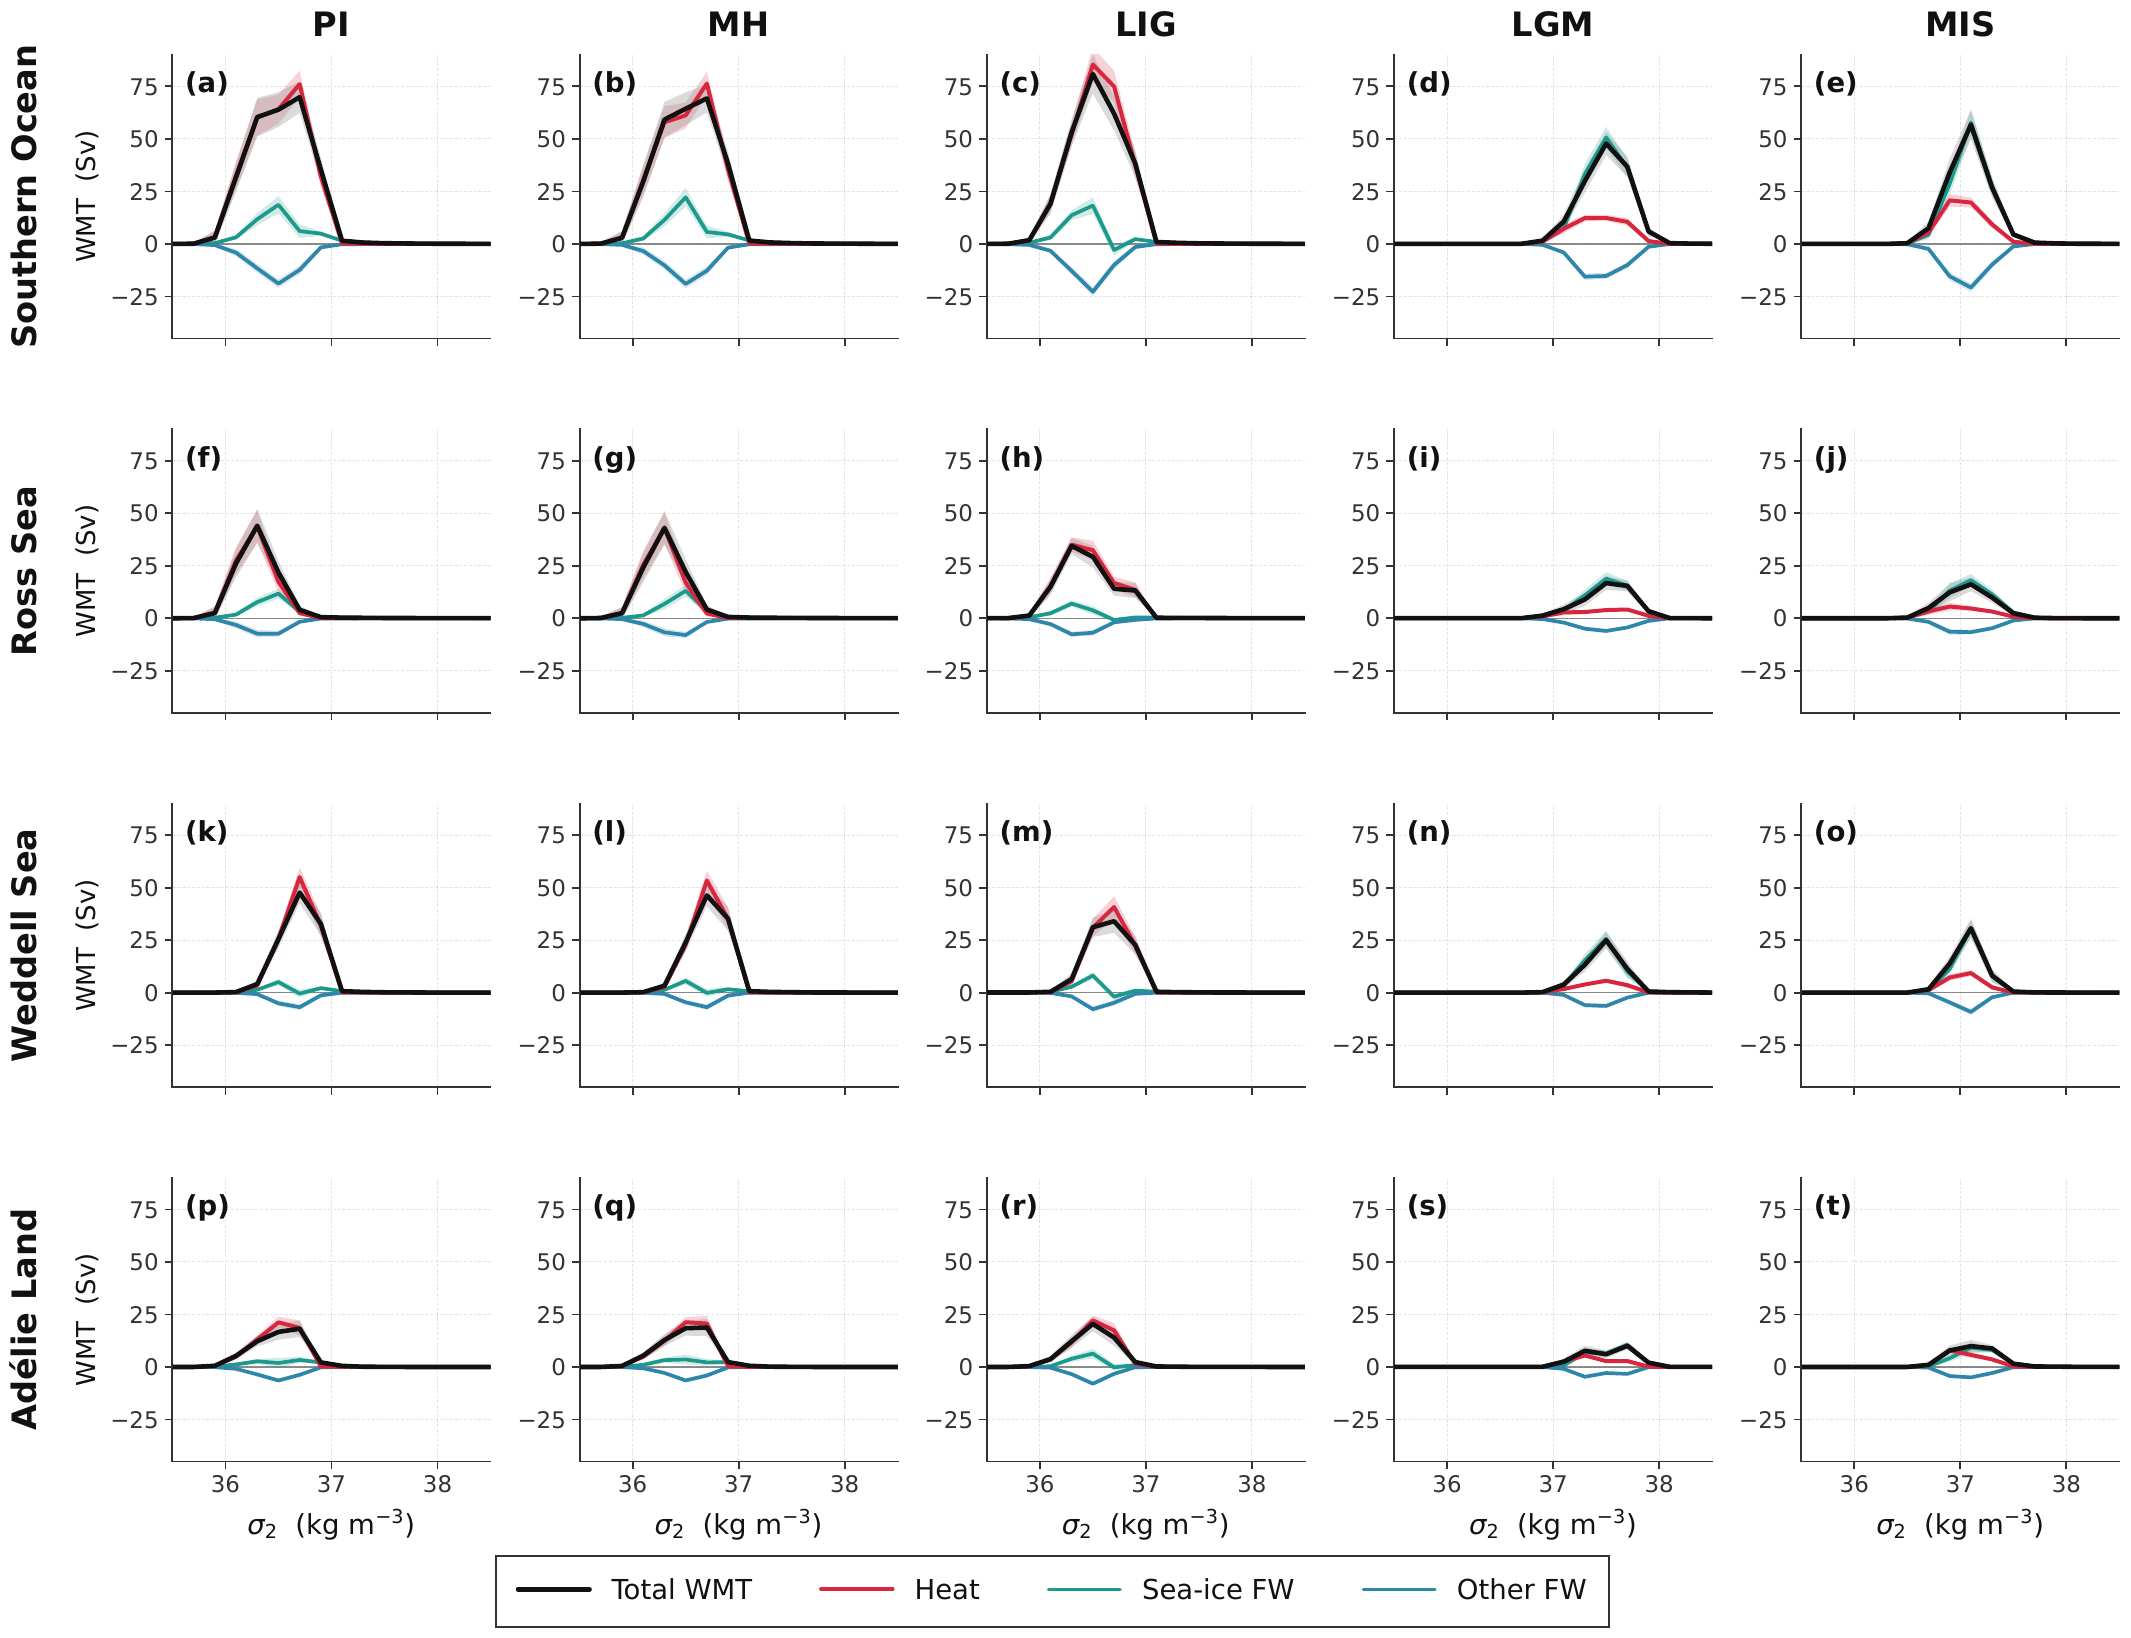
\includegraphics[width=\textwidth]{letter_figs/figS_common_axis-1.png}
\caption{\textbf{Figure R1.3} (new Supplementary Fig.~S5). Winter transformation for the
four sectors and five climate states on a common vertical and horizontal axis. Plotted this way the
glacial weakening of the transformation maximum and its shift to denser classes are directly
comparable between panels, which the independently scaled main-text version does not allow.\label{fig:r1axis}}
\end{figure}

16. Line 174: "Section 4?"If this is intended to refer to the Methods section

\medskip

\textcolor{blue}{\textbf{Corrected to refer to the Methods section by name.}}

\medskip

17. Fig.3 Please consider adding the climate-state labels at the top of each column, as in the other figures.

\medskip

\textcolor{blue}{\textbf{Added, here and on the other multi-panel figures. Reviewer 3 made the same request.}}

\medskip

18. Line 180/181: The LIG is first described as "showing modest changes", but later as "exhibiting a pronounced increase". These descriptions appear inconsistent.

\medskip

\textcolor{blue}{\textbf{The two statements referred to different quantities, which was not clear. The changes are
modest in the circumpolar integral and pronounced locally in the Ross Sea sector. The text now says
so explicitly.}}

\medskip

19. Could the authors briefly explain what is meant by thermal density tendency and sea-ice-driven density tendency in the methods.

\medskip

\textcolor{blue}{\textbf{Definitions have been added to the Methods:}}

\medskip

\textcolor{blue}{\textbf{	extit{``We refer throughout to the thermal density tendency, meaning the surface
density change produced by the net heat flux acting through the thermal expansion coefficient, and
to the sea-ice-driven density tendency, meaning the part of the haline term that is carried by the
thermodynamic growth and melt of sea ice. A positive value denotes densification of the surface
water in both cases. Brine released during ice growth increases surface salinity and therefore
density, whereas melting releases freshwater and reduces it.''}}}

\medskip

20. Line 209: Please add the appropriate reference(s) here to support this statement.

\medskip

\textcolor{blue}{\textbf{We now cite Cerove\v{c}ki et al. (2013) and Abernathey et al. (2016) in support of the
statement that turbulent rather than radiative fluxes control the surface buoyancy budget.}}

\medskip

21. Line216-246: Please refer to the relevant subpanels of Figure A5

\medskip

\textcolor{blue}{\textbf{Done.}}

\medskip

22. Line 249, 255: The phrase "across at high latitudes" is somewhat unclear. Does this refer specifically to the Antarctic coastal region or the Southern Ocean south of a particular latitude? Please consider rephrasing for clarity.

\medskip

\textcolor{blue}{\textbf{Both instances have been rewritten. They now read ``over the ice-free parts of the Southern
Ocean south of about 50$^\circ$S'' and ``south of the ice edge'' respectively.}}

\medskip

23. Could the authors clarify where the primary deep water formation regions occur in this model? Identifying these regions would also help assess whether the SAM-related changes shown in Figure 5 are directly influencing the main regions of dense water formation, as relatively little signal is apparent over the Weddell and Ross Seas.

\medskip

\textcolor{blue}{\textbf{We have added this diagnosis to the Results; it is shown in Fig.~\ref{fig:r1conv} above. In the
pre-industrial state the Weddell sector accounts for 70\% of the area with winter mixed layers
deeper than 400~m south of 55$^\circ$S and 97\% of the area deeper than 600~m, centred near
68$^\circ$S in the gyre interior. The formation region is therefore the open Weddell gyre rather
than the shelf. This also explains the pattern the reviewer noticed: the heat flux signal is
strongest over open water, and in the glacial states the coastal regions where dense water is
produced are precisely those insulated by ice, so the surface flux anomalies there are small even
though the transformation response is not.}}

\medskip

24. Lines 261-263: Please consider expanding on the physical mechanism linking positive SAM to freshwater loss and intensified brine rejection by additional explanation and supporting references.

\medskip

\textcolor{blue}{\textbf{Expanded, with the mechanism stated as a sequence: strengthened and poleward-shifted westerlies
increase offshore Ekman transport of sea ice, which opens coastal polynyas, which exposes water at
the freezing point to the atmosphere and sustains rapid new ice growth, which concentrates brine
locally while the exported ice carries the compensating freshwater away to melt further north.
References added.}}

\medskip

25. Line 291, 294: Please check citation format

\medskip

\textcolor{blue}{\textbf{Corrected.}}

\medskip

26. Line 301:Figure A4 appears to show only model results. Please consider including the observational estimates in the figure (or referring to them directly) to support this statement. As noted above, it would also improve readability if the appendix figures were cited in numerical order.

\medskip

\textcolor{blue}{\textbf{We have added the quantitative comparison to the text and to the new Fig.~8, reproduced as
Fig.~\ref{fig:r1domain} above. We report the published values directly in the Discussion, including
the 5~$\pm$~5~Sv transformation into denser classes and the stated factor of 2--5 by which the
freshwater term exceeds the heat term in their sector, and compare our numbers against them. We
chose to make the comparison quantitatively in the text and in a dedicated figure rather than
overplotting their curve, because their analysis is in neutral density over a different density
range and an overlay would misleadingly imply a point-by-point correspondence that does not exist;
the density-range mismatch is itself one of our findings. The appendix figures are now also cited in
numerical order.}}

\medskip

27. Lines 308-321: The discussion quantifies the interglacial changes (e.g., lines 315-316), but similar quantification is not provided for the glacial changes. For consistency, please consider including quantitative estimates for both.

\medskip

\textcolor{blue}{\textbf{Added. The glacial transformation maximum weakens to below 60~Sv and moves to
$\sigma_2 = 37.0$--$37.5$~kg~m$^{-3}$, with the thermal share falling to 12--17\%. In the revised manuscript this now reads: \textit{``The winter transformation maximum weakens to below 60 Sv and moves to \_2 = 37.0-37.5 kg m$^{-3}$, and the thermal share of the transformation falls to 12-17\% while the sea ice term becomes dominant. Extensive ice cover insulates the ocean from atmospheric heat exchange, and simultaneously intensifies haline forcing through enhanced brine rejection concentrated in coastal regions.''}}}

\medskip

28. Lines 326 appear to repeat the statement made in line 323. In addition, the general statement in lines 323-325 does not appear to hold equally across all climate states. For example, the Ross Sea and Weddell Sea exhibit different behaviour for the peak-density classes.

\medskip

\textcolor{blue}{\textbf{The repetition has been removed by merging the two sentences. We have also added the
qualification the reviewer asks for, noting that the Ross Sea departs from the circumpolar picture
and that in the glacial states the signal is carried largely by the Weddell sector. In the revised manuscript this now reads: \textit{``This circumpolar picture does not hold uniformly in every sector. The Ross Sea in particular departs from it, showing weaker and at some densities opposing responses, and in the glacial states the circumpolar signal is carried largely by the Weddell sector while the Ross and Adelie sectors contribute little.''}}}

\medskip

29. Line 339: Please provide a reference for the sediment-record evidence discussed here.

\medskip

\textcolor{blue}{\textbf{On reflection we think the passage was speculative rather than supported, and Reviewer 3 raised
the same objection from the opposite direction, noting that accumulation rates around the Antarctic
margin are very low. We have therefore replaced the proposal with a statement of the difficulty,
and now present the persistence of the coupling as a property of the simulated system rather than as
a practical route to a marine reconstruction.}}

\medskip

30. Section 4.1: Please define the full names of the abbreviated components

\medskip

\textcolor{blue}{\textbf{Done. The Methods now spell out that the radiative component is the sum of the shortwave and
longwave fluxes and the turbulent component the sum of the latent and sensible heat fluxes. In the revised manuscript this now reads: \textit{``In the figures the radiative component denotes the sum of the shortwave and longwave fluxes, and the turbulent component denotes the sum of the latent and sensible heat fluxes.''}}}

\medskip

31. Line 388: Please check the citation formatting.

\medskip

\textcolor{blue}{\textbf{Corrected.}}

\medskip

32. Lines 394-403: Please consider including a summary table listing the prescribed boundary conditions for each experiment (e.g., greenhouse gas concentrations, orbital parameters, ice-sheet reconstruction, and any other relevant forcings). This would make the experimental setup considerably easier to follow.

\medskip

\textcolor{blue}{\textbf{Added as Table~1 of the revised manuscript; please see our reply to the general comment on
boundary conditions above.}}

\medskip

\clearpage


\section*{Reviewer \#2}

\medskip

General

This study uses the Water Mass transformation (WMT) framework to perform an analysis of the buoyancy forcing in the Southern Ocean under conditions corresponding to paleo scenarios (Last glacial maximum, Pre-industrial, also MIS3 and mid-Holocene). It uses a single model, the AWI-ESM.

The model is quite impressive in that it gets a believable-looking circulation for the glacial simulations, with dense AABW that has an old ventilation age, and the main point of the paper is that this is achieved by a shift from thermally-driven bouyancy forcing in the Southern Ocean under inter-glacial situations, to freshwater-salt-driven by ice formation processes in glacial times.

Though the WMT analysis was introduced over 40 years ago, it has enjoyed renewed attention more cecently. It has been increasingly used for novel studies and tools have become available to apply it to numerical model outputs, decomposing them into haline and thermal forcing. This is the first time I have seen it used in the context of a paleo model and potentially it adds explanatory power to the narrative of increased sea-ice buoyancy forcing in glacial time.

So in principle this is an interesting and topical paper and I would like to be able to support its publication. However, I have two big issues with the present MS that in my view mean it needs at least some substantial revision.

\medskip

\textcolor{blue}{\textbf{We are grateful for both issues, which were well aimed, and we address them in turn
below.}}

\medskip

\subsection*{Major issue 1}

\medskip

1) There is a mismatch with observational studies of the modern ocean. In their model the pre-industrial situation is dominated by thermal buoyancy forcing whereas Pellichero et al, (2018) find the opposite: The title of their observation-based paper makes this clear: "Southern Ocean meridional overturning is driven by freshwater fluxes". Shi et al dismiss this difference in a single sentence, saying it is due to "model biases or regional differences in analysis domains" (line 305). Comparing their Fig 3a, Fig 4a with Pellichero Fig 2a and c, the regions look similar, suggesting it's mostly model bias. But the switch from thermal to haline forcing is the present paper's main result, so if indeed it is due to model bias, this seems like a major problem.

\medskip

\textcolor{blue}{\textbf{The reviewer is right that the original single sentence was inadequate, and right to
insist that the answer matters for the paper's main claim. We therefore tested it directly rather
than speculating. Three findings emerged, and we report all three, including the one that is
unfavourable to us.}}

\medskip

\textcolor{blue}{\textbf{\textbf{The domains are less similar than they appear.} Pellichero et al. define their
sector as the region enclosed by the September 15\% sea ice contour, so its northern boundary is an
ice contour that varies with longitude, not a latitude circle. Our published integral covers
everything south of 60$^\circ$S. In our pre-industrial simulation, 42.7\% of that area lies outside
the September ice contour and is therefore water their analysis does not include. It is also the
part of the domain that stays exposed to the atmosphere year round, and taken alone it is 89--91\%
thermally driven in the dense classes. Recomputing our transformation over a sea ice sector defined
exactly as theirs, which reproduces their domain to within 2.5\% in area, moves the partition in the
direction they report: the thermal share of the dense-class transformation falls from 69\% to 61\%,
and the sea ice contribution at the transformation maximum roughly doubles from 0.86 to 1.84~Sv.}}

\medskip


\begin{figure}[htbp]
\centering
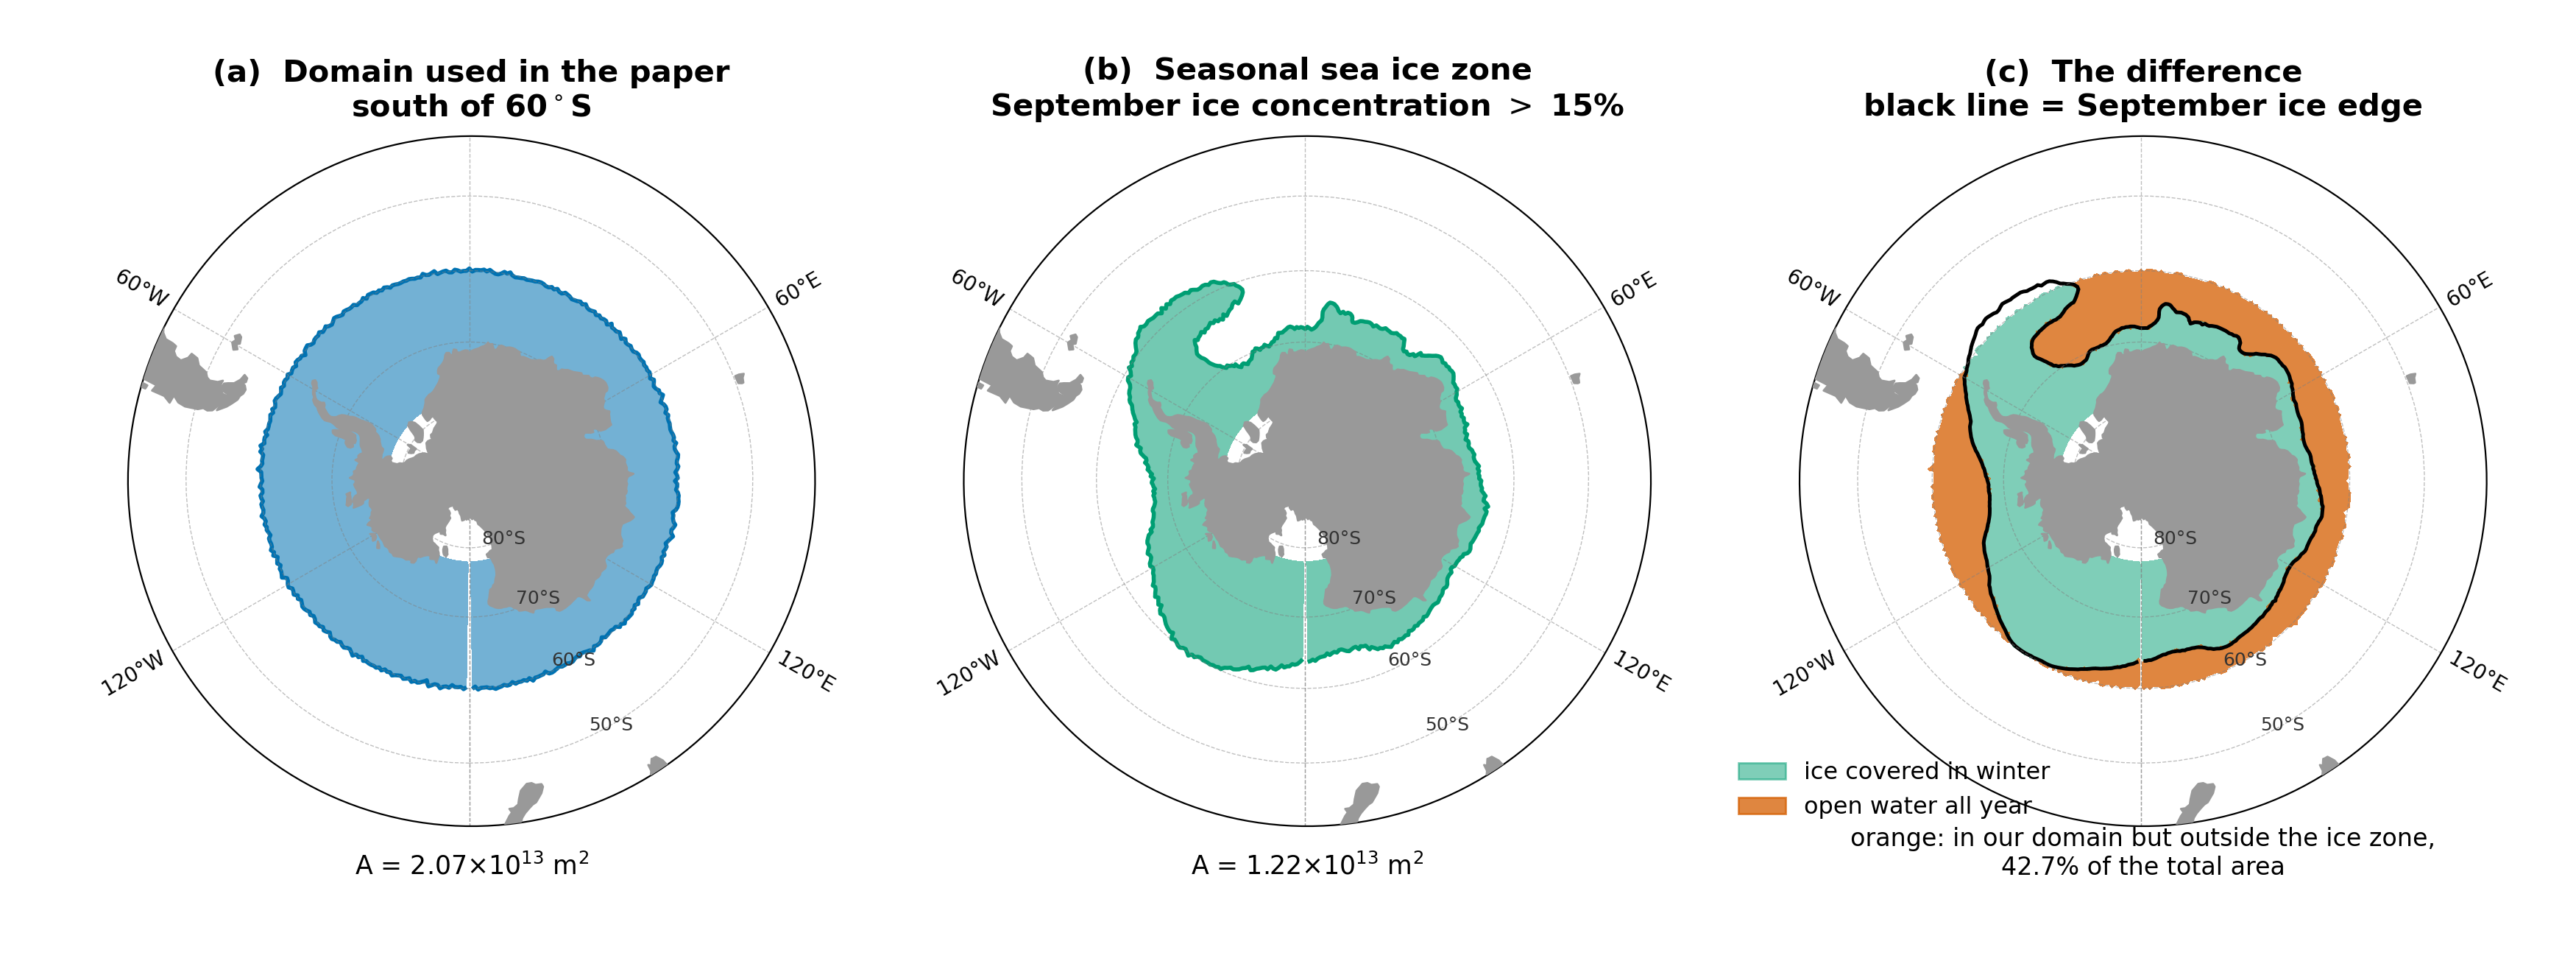
\includegraphics[width=\textwidth]{letter_figs/figR8_domain_map.png}
\caption{\textbf{Figure R2.1} (new analysis). (a) The domain used in the submitted manuscript,
everything south of 60$^\circ$S, covering 2.07$\times10^{13}$~m$^2$. (b) The seasonal sea ice zone
of the model, inside the September 15\% contour, which is the definition Pellichero et al. use,
covering 1.22$\times10^{13}$~m$^2$. (c) The two overlaid. The orange ring lies inside our domain but
outside the ice zone: it is 42.7\% of the area we integrated over, it is open water all year, and it
is water their analysis does not include.\label{fig:r2map}}
\end{figure}


\begin{figure}[htbp]
\centering
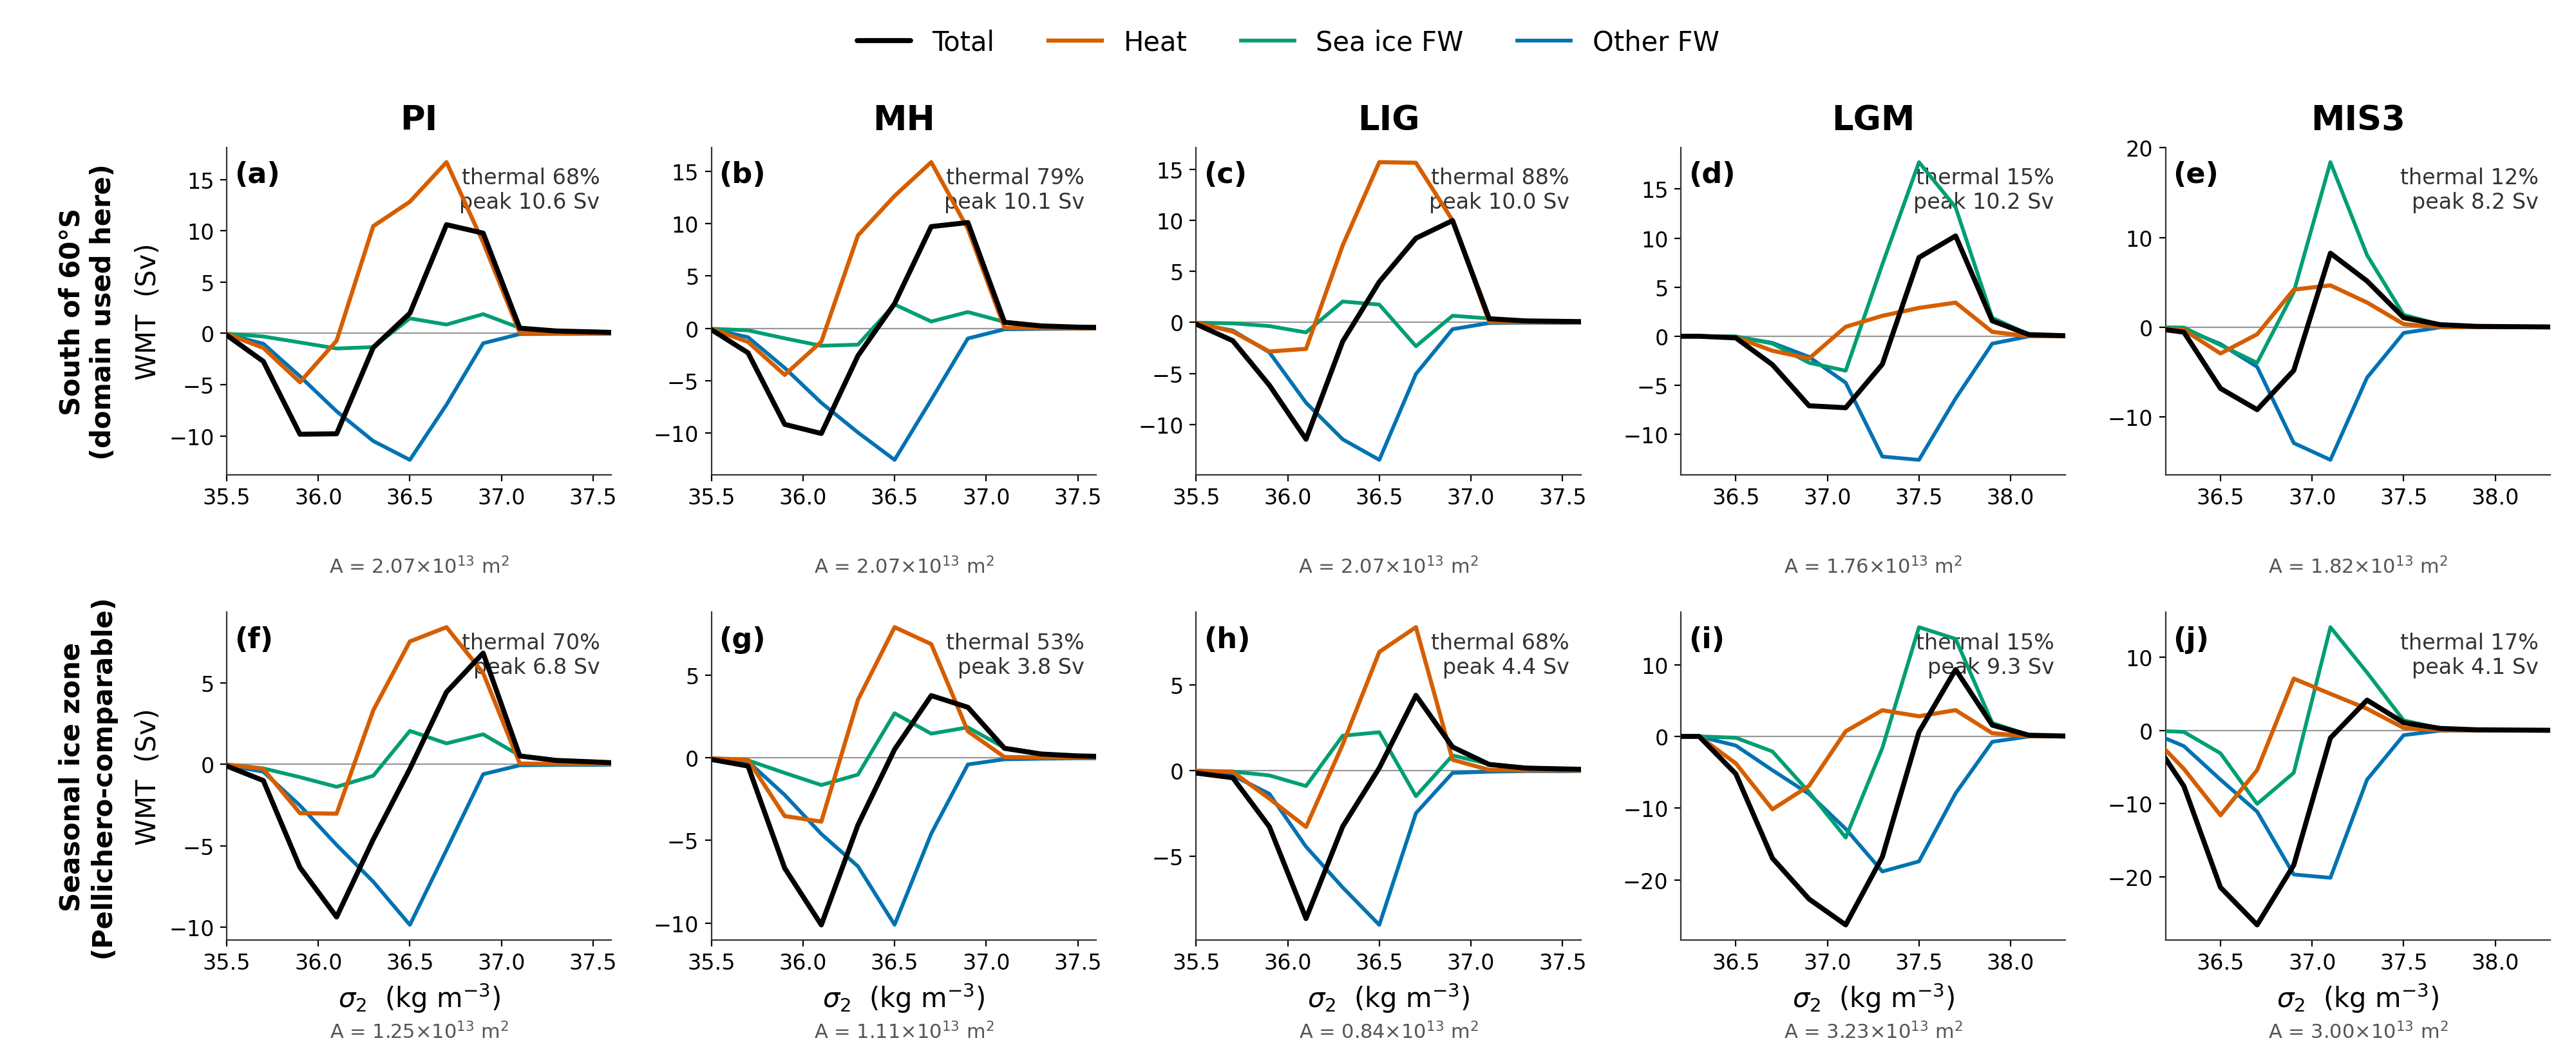
\includegraphics[width=\textwidth]{letter_figs/figR1_wmt_domain_sensitivity.png}
\caption{\textbf{Figure R2.2} (manuscript Fig.~8). Transformation integrated south of
60$^\circ$S, the domain used in the submitted version (top row), and over the seasonal sea ice zone
alone, which reproduces the domain of Pellichero et al. (2018) to within 2.5\% in area (bottom row).
Restricting the integration to the ice-covered sector raises the haline share, as the reviewer would
expect, but the contrast between thermally dominated interglacials and haline dominated glacials
survives intact.\label{fig:r2domain}}
\end{figure}

\textcolor{blue}{\textbf{\textbf{The density range matters more than the domain.} This was the more
consequential finding. Converting our simulated surface properties inside the September ice zone to
the neutral density coordinate that Pellichero et al. use, our thermally dominated transformation
maximum sits near $\gamma_n \approx 27.3$~kg~m$^{-3}$, whereas the haline-dominated lower cell they
describe occupies $\gamma_n = 27.9$--$28.8$~kg~m$^{-3}$. Our simulated surface transformation barely
reaches the lighter edge of their range. In the densest classes our fluxes do populate
($\sigma_2 \ge 37.0$~kg~m$^{-3}$), our pre-industrial transformation is haline dominated, with
0.79~Sv from sea ice against 0.06~Sv from heat. The two analyses are therefore largely describing
different water masses, ours weighted toward mode and intermediate densities and theirs toward
bottom water densities, and where they overlap they agree in sign.}}

\medskip

\textcolor{blue}{\textbf{\textbf{A residual discrepancy remains, and it is genuine model bias.} We can rule out
one candidate explanation. Pellichero et al. attribute part of the haline dominance to the thermal
expansion coefficient being near zero at the freezing point, so we checked whether our ice-covered
sector reproduces that regime. It does: the area-weighted winter surface temperature inside the
September ice zone is $-1.08$~$^\circ$C, the median is $-1.71$~$^\circ$C, 55\% of the area lies
within 0.5~$^\circ$C of the local freezing point, and $\alpha = 3.5\times10^{-5}$~K$^{-1}$. The model
is not warm-biased there, so we cannot appeal to that. What differs is where dense water is made.}}

\medskip


\begin{figure}[htbp]
\centering
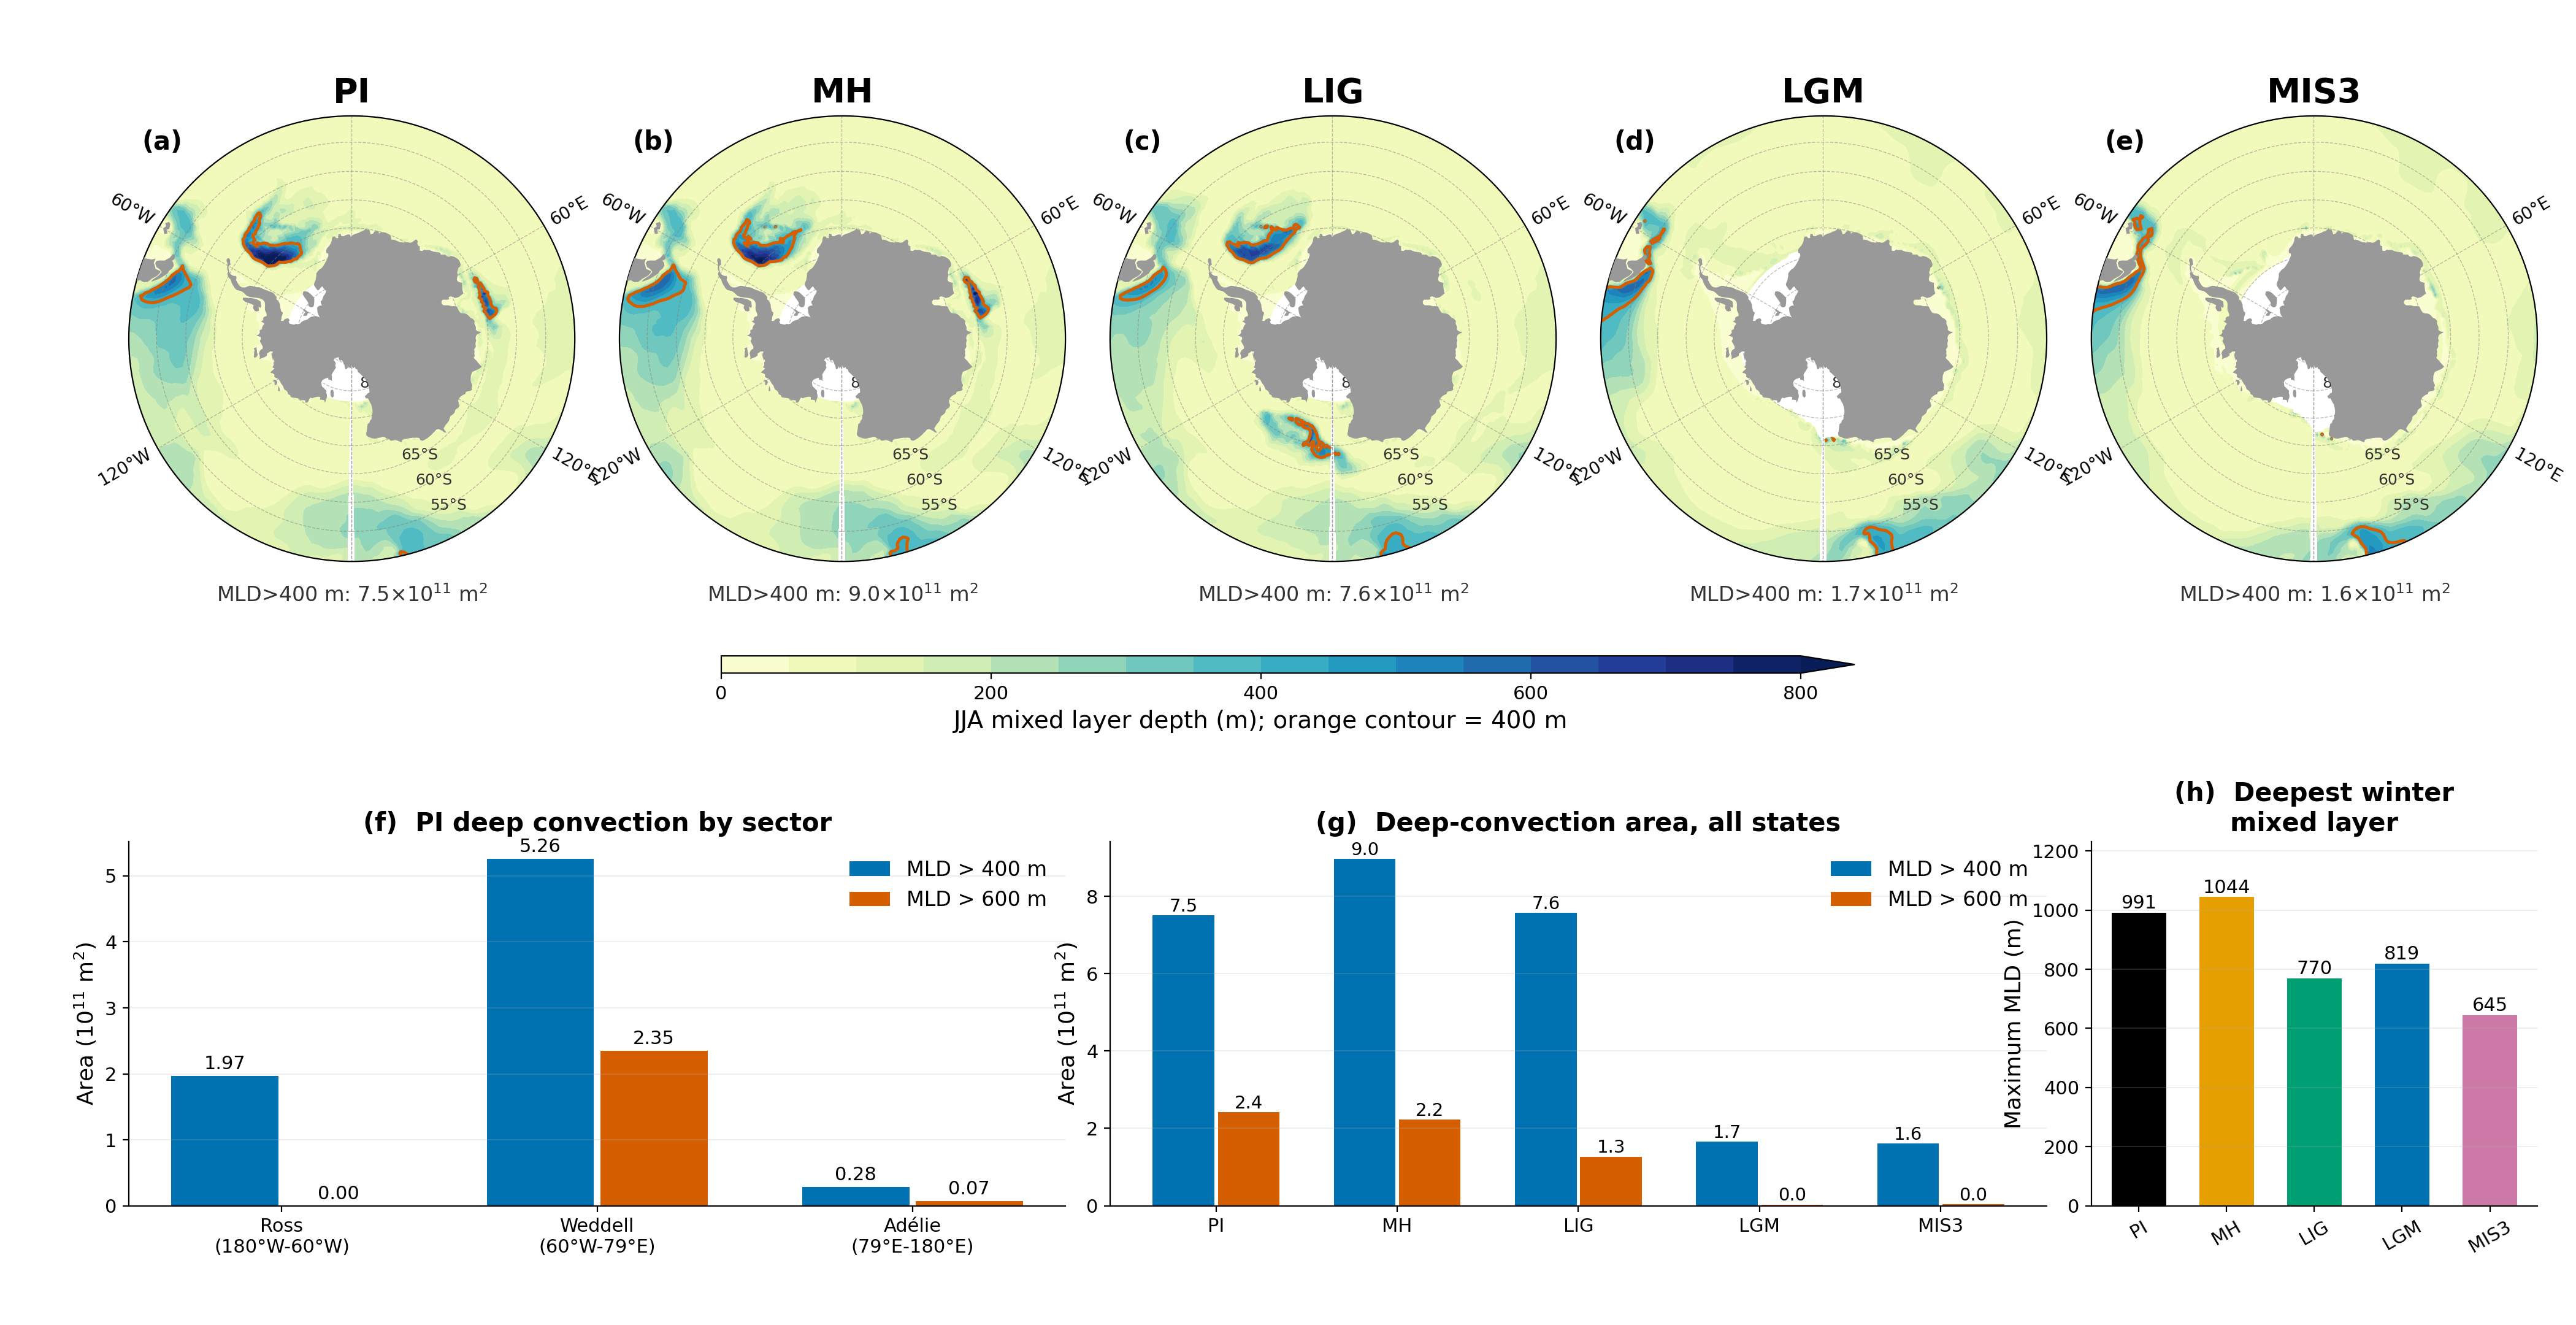
\includegraphics[width=\textwidth]{letter_figs/figR6_convection_sites.png}
\caption{\textbf{Figure R2.3} (new analysis). Where the model actually convects. (a--e) Winter
mixed layer depth, 400~m contour in orange. (f) In the pre-industrial state 70\% of the area with a
mixed layer deeper than 400~m, and 97\% of the area deeper than 600~m, lies in the Weddell sector,
centred near 68$^\circ$S in the open gyre rather than over the shelf. (g, h) The deep-convection
area and the maximum mixed layer depth both contract sharply in the glacial states.\label{fig:r2conv}}
\end{figure}

\textcolor{blue}{\textbf{Open-ocean convection exposes a large area to the atmosphere and so recruits an
excessive thermal contribution while producing water that is not dense enough, which is precisely
the offset in density class described above. We now say this plainly in the Discussion, note that it
is a limitation shared across the current model generation rather than specific to AWI-ESM2
(Heuz\'e, 2021: 28 of 35 CMIP6 models), and state that this configuration has no ice shelf
cavities.}}

\medskip

\textcolor{blue}{\textbf{\textbf{Does the main result survive?} We think it does, for two reasons that we now
give in the text. First, the regime shift survives the domain test. Recomputed over the sea ice
sector alone, the glacial states remain 15\% and 17\% thermally driven while the interglacials remain
53--88\% thermally driven, so the contrast is not manufactured by including open water in the
interglacial integrals. Second, the mechanism is the ice cover itself rather than the convection
style: insulation of the surface and concentration of brine rejection follow from the areal
expansion of sea ice, and both would operate in a model that formed its dense water on the shelf.
What such a model would change is the density and the geographic origin of the resulting water, not
the direction of the shift in the surface buoyancy budget. The consequences for the large-scale
circulation are visible in the overturning itself.}}

\medskip


\begin{figure}[htbp]
\centering
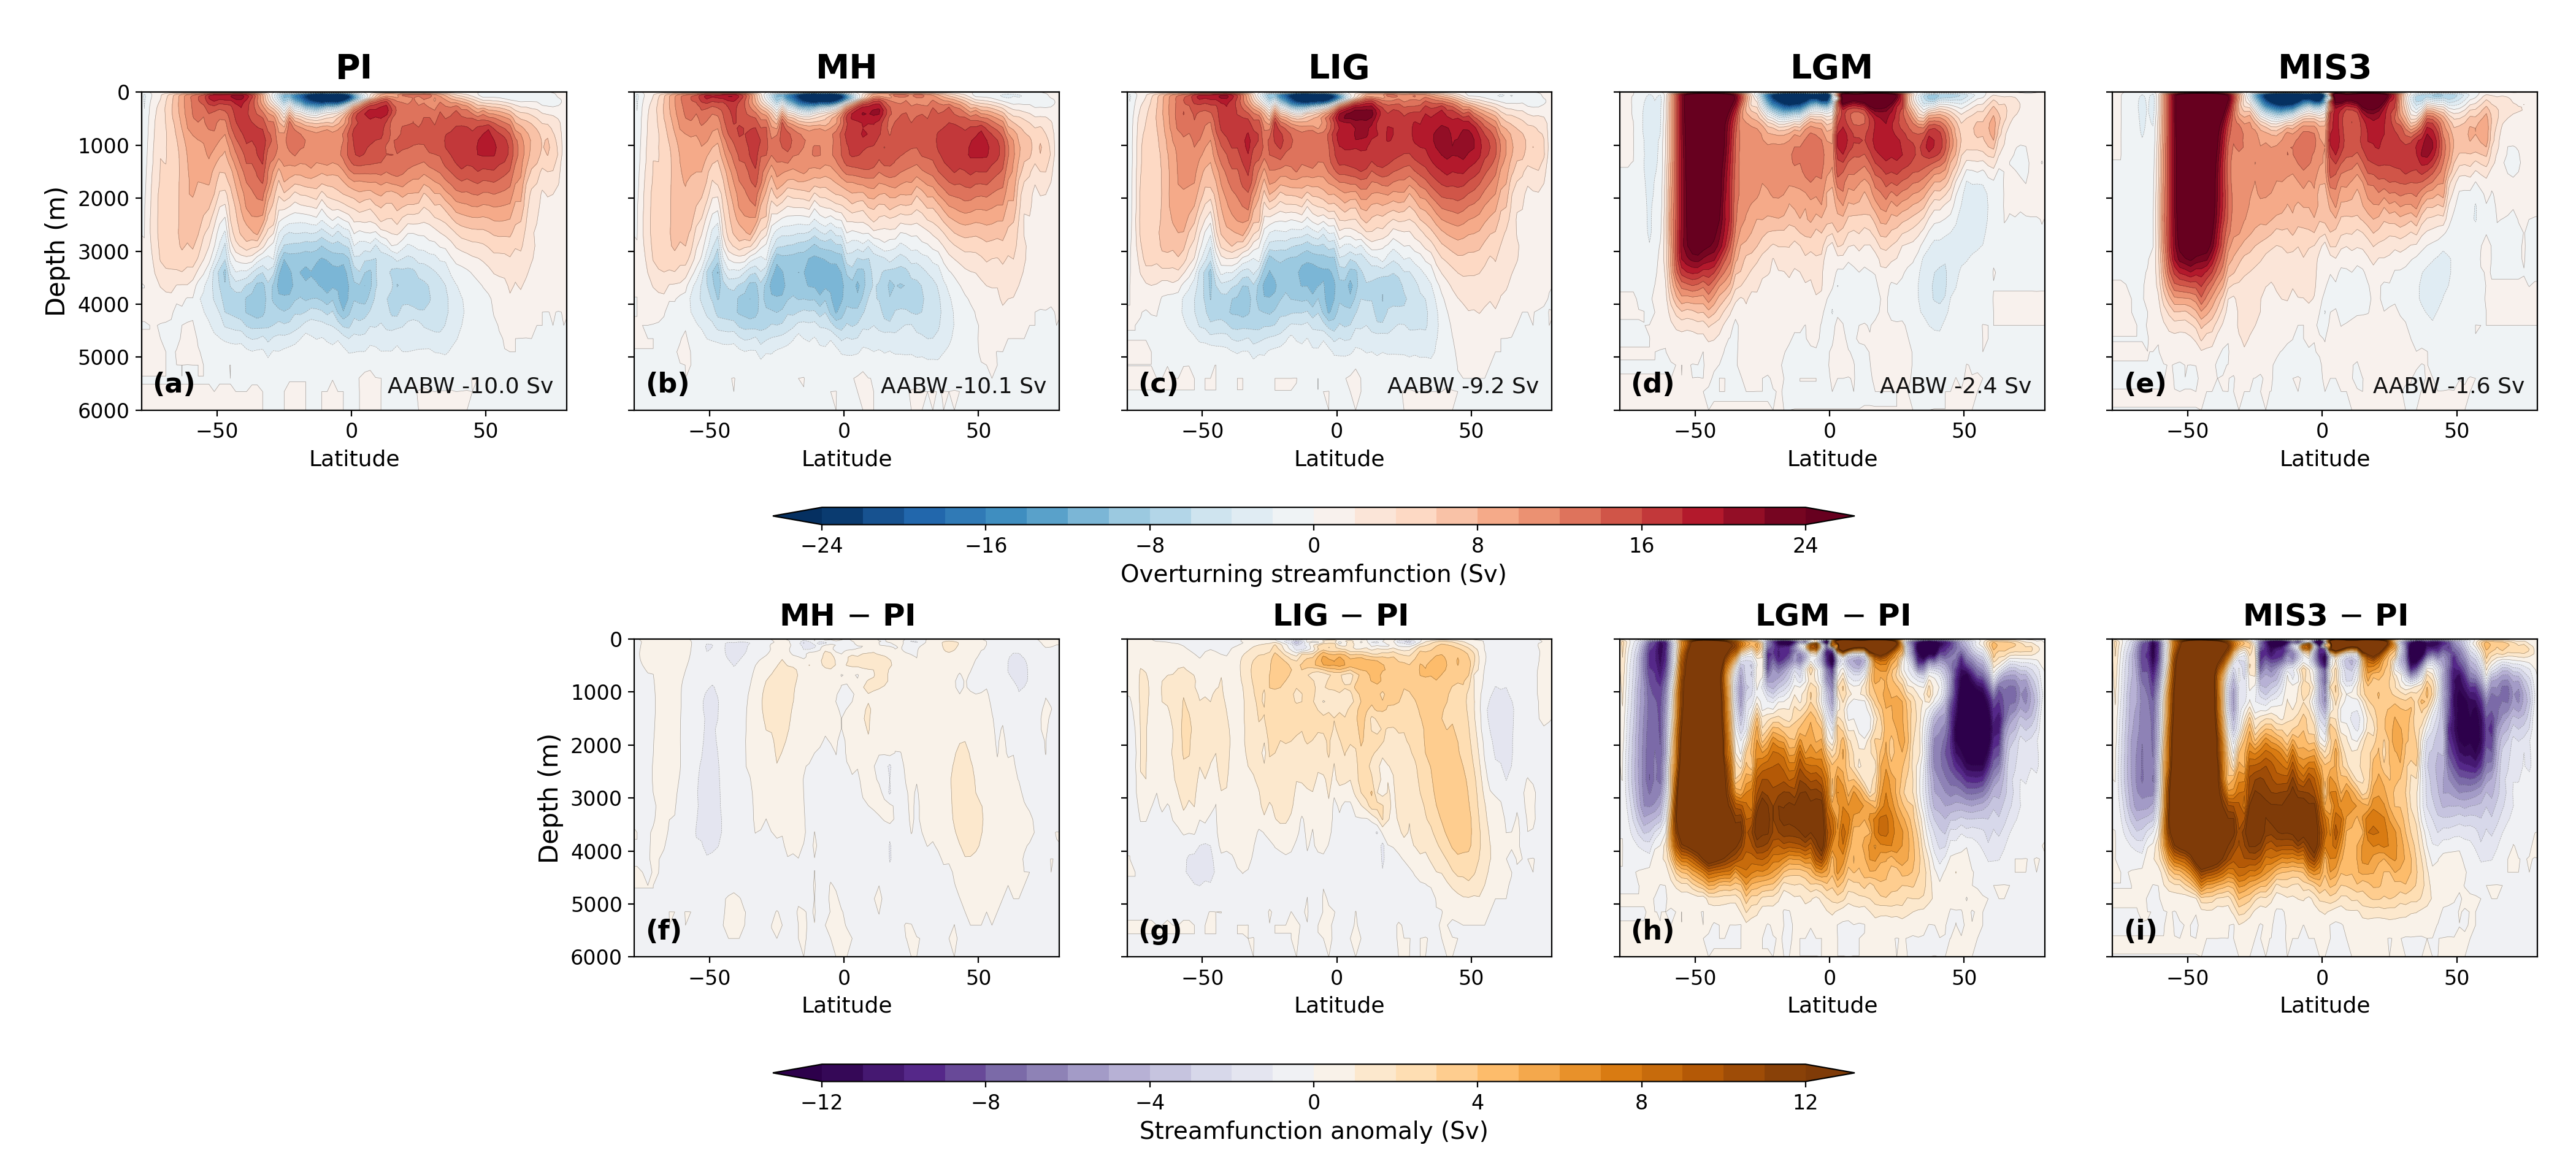
\includegraphics[width=\textwidth]{letter_figs/figR2_moc_5exps.png}
\caption{\textbf{Figure R2.4} (manuscript Fig.~6). Global overturning streamfunction (top) and
anomalies relative to PI (bottom). The abyssal cell that carries southern-sourced bottom water
weakens from about 10~Sv in the interglacials to 2.4 and 1.6~Sv in LGM and MIS3, while the upper
cell is largely unchanged. The glacial reorganisation is concentrated in the cell our surface
analysis addresses.\label{fig:r2moc}}
\end{figure}

\textcolor{blue}{\textbf{We have adjusted the framing of the paper accordingly, so that the claim is about the
partitioning of surface buoyancy forcing and its state dependence rather than about bottom water
formation rates.}}

\medskip

\subsection*{Major issue 2}

\medskip

2) I'm puzzled that they don't acknowledge or discuss the relation of their work with recent studies showing very similar results but analysed through different tools and language. Using the same ocean model Chen et al, 2025 (GRL 52, e2025GL114809) describe formation of very dense AABW in glacial time as due to the enhanced ice formation, where the resulting water mixes more slowly with overlying waters due to the greater density difference. One of the authors (Lohmann) is on both papers, yet this paper is not referenced, let alone discussed, by Shi et al. I ask myself what is learned from the WMT analysis that is not already discussed in that paper?

\medskip

\textcolor{blue}{\textbf{The omission was an oversight on our part and we apologise for it. The paper is now
cited in both the Introduction and the Discussion, and we address the reviewer's question directly
rather than merely adding the reference.}}

\medskip

\textcolor{blue}{\textbf{We first acknowledge the genuine agreement. Chen et al. attribute the large glacial
volume of Atlantic bottom water to a substantial increase in sea ice export toward lower latitudes,
which supplies dense shelf water year round, and to weaker mixing between northern- and
southern-sourced water, which lets that water retain the properties of its origin. Our glacial
conclusions are consistent with theirs, and we say so explicitly rather than presenting our result
as new in that respect.}}

\medskip

\textcolor{blue}{\textbf{What the transformation analysis adds is of two kinds. The first is measurement rather
than inference. Chen et al. diagnose water mass volumes, the overturning streamfunction, and
mixed-layer and sea ice fields, from which the role of sea ice is inferred because those fields
covary with it. A decomposed surface buoyancy budget measures the transformation directly and
attributes it to individual flux components in sverdrups, so the sea ice contribution is quantified
rather than inferred. Our analysis therefore tests the mechanism they proposed, and finds it
supported.}}

\medskip

\textcolor{blue}{\textbf{The second is scope. Their simulations are ocean-only, with a prescribed atmosphere,
and cover the Last Glacial Maximum and the present day. Ours are fully coupled, so sea ice and the
atmospheric fluxes evolve together, and they span five climate states. A shift between two forcing
regimes cannot be identified from a single glacial state; it requires the interglacial end members
for the contrast to exist at all. The regime shift that is our central result is therefore not
addressable within their experimental design, which is why the two studies reach compatible
conclusions about the glacial ocean while answering different questions. We have phrased this in the
manuscript as the present analysis testing and quantifying the mechanism Chen et al. proposed,
rather than as a claim that they missed something.}}

\medskip

\subsection*{More minor points}

\medskip

The fundamental issue must be getting right the formation of sea ice and rejection of brine close to the continent, followed by the mixing of that dense water with the surroundings, all processes that intrinsically occur at fine spatial scales. In this regard the model looks good, by comparison to most paleo studies. The comparatively high resolution close to the continent must be helpful I'm sure, (though at 25 km it may still not be enough to realistically model the dynamics of polynya formation and brine rejection). Some more information on just how this is being managed would add to the value of the paper.

\medskip

\textcolor{blue}{\textbf{We agree with the reviewer's caveat and have expanded the Methods accordingly:}}

\medskip

\textcolor{blue}{\textbf{	extit{``At this resolution the larger coastal polynyas are represented as features, but the
boundary layer processes that set polynya dynamics are not resolved. Sea ice growth and melt are
computed thermodynamically at each surface node, and the associated brine release enters the ocean
as a salt flux at that node, so the brine signal appears wherever the model forms ice; its
intensity, however, depends on the simulated wind-driven ice divergence rather than on a resolved
polynya circulation. The configuration does not include ice shelf cavities, so the ocean beneath
floating ice shelves, and the basal melt it supplies, are absent from the simulations.''}}}

\medskip

The authors highlight the lack of deep convection in the glacial open ocean due to the very extensive winter-time ice cover. A little more discussion of how/why the model achieves this ice cover would be welcome, as previous paleo-model studies often don't get that, and as a result may have too much deep convection in glacial simulations, which doesn't match so well with paleo-proxies. (Another paper they don't cite is Lhardy, Climate of the Past, 17, 1139-1159, 2021, which discusses how most PMIP models fail in this regard.)

\medskip

\textcolor{blue}{\textbf{Thank you for this reference, which we have added and discussed. We now note that
maintaining an extensive glacial ice cover is not a general feature of paleoclimate simulations,
that many PMIP models underestimate glacial Southern Ocean sea ice and its seasonality, and that
colder glacial forcing on its own tends to intensify open-ocean convection rather than suppress it,
so that better boundary conditions do not by themselves fix the problem. We highlight the finding of
Lhardy et al. that the only configuration avoiding an unrealistically deep northern-sourced cell was
the one in which brine sinking along the Antarctic margin was parameterised explicitly. In our
simulations the glacial ice expands sufficiently to insulate the interior gyres, and the area of
deep winter mixed layers contracts to roughly one fifth of its pre-industrial value
(Fig.~\ref{fig:r2conv}g). We now state that our glacial result depends on that simulated expansion
being realistic, and that while proxy reconstructions support the direction of the change, the
quantitative agreement remains uncertain.}}

\medskip

In Results section 2.1 the acronyms (MH, LIG etc) are used without introduction. They are defined later, section 4, but as the paper is laid out this is not obvious to the reader coming to section 2.

\medskip

\textcolor{blue}{\textbf{Corrected. The five experiments and their abbreviations are now introduced at the
start of the Results, at first use, in addition to the Methods definition. Reviewer 3 made the same
point.}}

\medskip

The discussion of the role of the effects of the SAM is interesting, but could I think be shortened, since it is somewhat secondary to the main messages of the paper. Figs 5 and 6 could be moved to the supplementary information.

\medskip

\textcolor{blue}{\textbf{We have done this. All of the Southern Annular Mode figures, including Figs 5 and 6,
have been moved to the Supplementary Information, so the main text no longer carries any figure
devoted to the mode. We have also shortened the section, removing the repetition that Reviewer 1
flagged and cutting the speculative passage about marine proxy reconstruction. What remains in the
main text is a compact account of the result, with the supporting composites available to readers
who want them. We note that Reviewer 3 took the opposite view of this material, describing it as the
more generalisable part of the study. Moving the figures to the supplement while keeping a concise
statement of the result in the main text seemed to us the arrangement most likely to satisfy both
readings.}}

\medskip

For figs 5 and 6, I think it would be helpful if the forcings were on the same equivalent scales of buoyancy anomaly -- currently they are in different units and it is impossible to see how they compare in absolute values.

\medskip

\textcolor{blue}{\textbf{This is a fair criticism. We have added a statement of the comparison in equivalent
surface density tendency terms to the Results: expressed that way, the freshwater contribution is
the larger of the two wherever sea ice is present, and the heat contribution is larger only in the
ice-free sector, which is the same partition that governs the mean state. We have kept the native
units in the figures themselves, which are now supplementary, because the heat and freshwater fields
are what the model diagnoses and readers may wish to compare them against other studies in
conventional units. If the reviewer would prefer the figures recast in buoyancy units, we will do
so.}}

\medskip

\clearpage


\section*{Reviewer \#3}

\medskip

Shi et al apply a water mass transformation (WMT) framework to various glacial/interglacial paleoclimate sims using AWI-ESM2. This is an interesting framework for thinking about mechanisms of deepwater formation and how production regimes may shift between climate states, and a novel application. The results indicate the density transformation shifts from a thermal to salt regime between glacial and interglacial states. The observation that the reduction in buoyancy loss through atmospheric heat loss from enhanced sea ice cover is compensated by increased buoyancy loss via sea ice export, is an interesting result and points to an interesting stabilising mechanism for ventilation.

\medskip

\textcolor{blue}{\textbf{We thank the reviewer for this reading, and particularly for identifying the
compensation mechanism as the interesting result, which has helped us frame the revision.}}

\medskip

While this is an interesting observation in model space, with potential interest for thinking about paleoclimates, the major issue I currently see for the current framing of the manuscript (and mentioned by the authors on lines 291-297) is that to the best of our knowledge today densewater formation in the Southern Ocean is not primarily a thermally driven regime. Like many models, AWI-ESM2 appears to form AABW via open ocean convection under PI conditions whereas in the real ocean AABW is largely a salt/freshwater controlled process occurring on the shelves (e.g. Orsi et al 1999).

Today AABW forms on shelves via interaction with ice cavity melting and coastal polynyas. Upwelling warm CPDW melts basal ice, which cools the shelf water to insitu freezing point but substantially freshens it (e.g. Toggweiler 1995). This close to freezing shelf water then looses further buoyancy in coastal polynas via brine rejection, and flows downslope off the shelves via gravity currents. This must be the starting point for thinking about glacial changes, not thermally driven open ocean convection, unless the authors believe this is somehow an overlooked process in the real modern ocean*.

\medskip

\textcolor{blue}{\textbf{We accept this criticism. We do not believe shelf processes are overlooked in the real
ocean, and we have restructured the Discussion so that the model's convection behaviour is stated at
the outset rather than left implicit. We confirmed the reviewer's suspicion diagnostically.}}

\medskip


\begin{figure}[htbp]
\centering
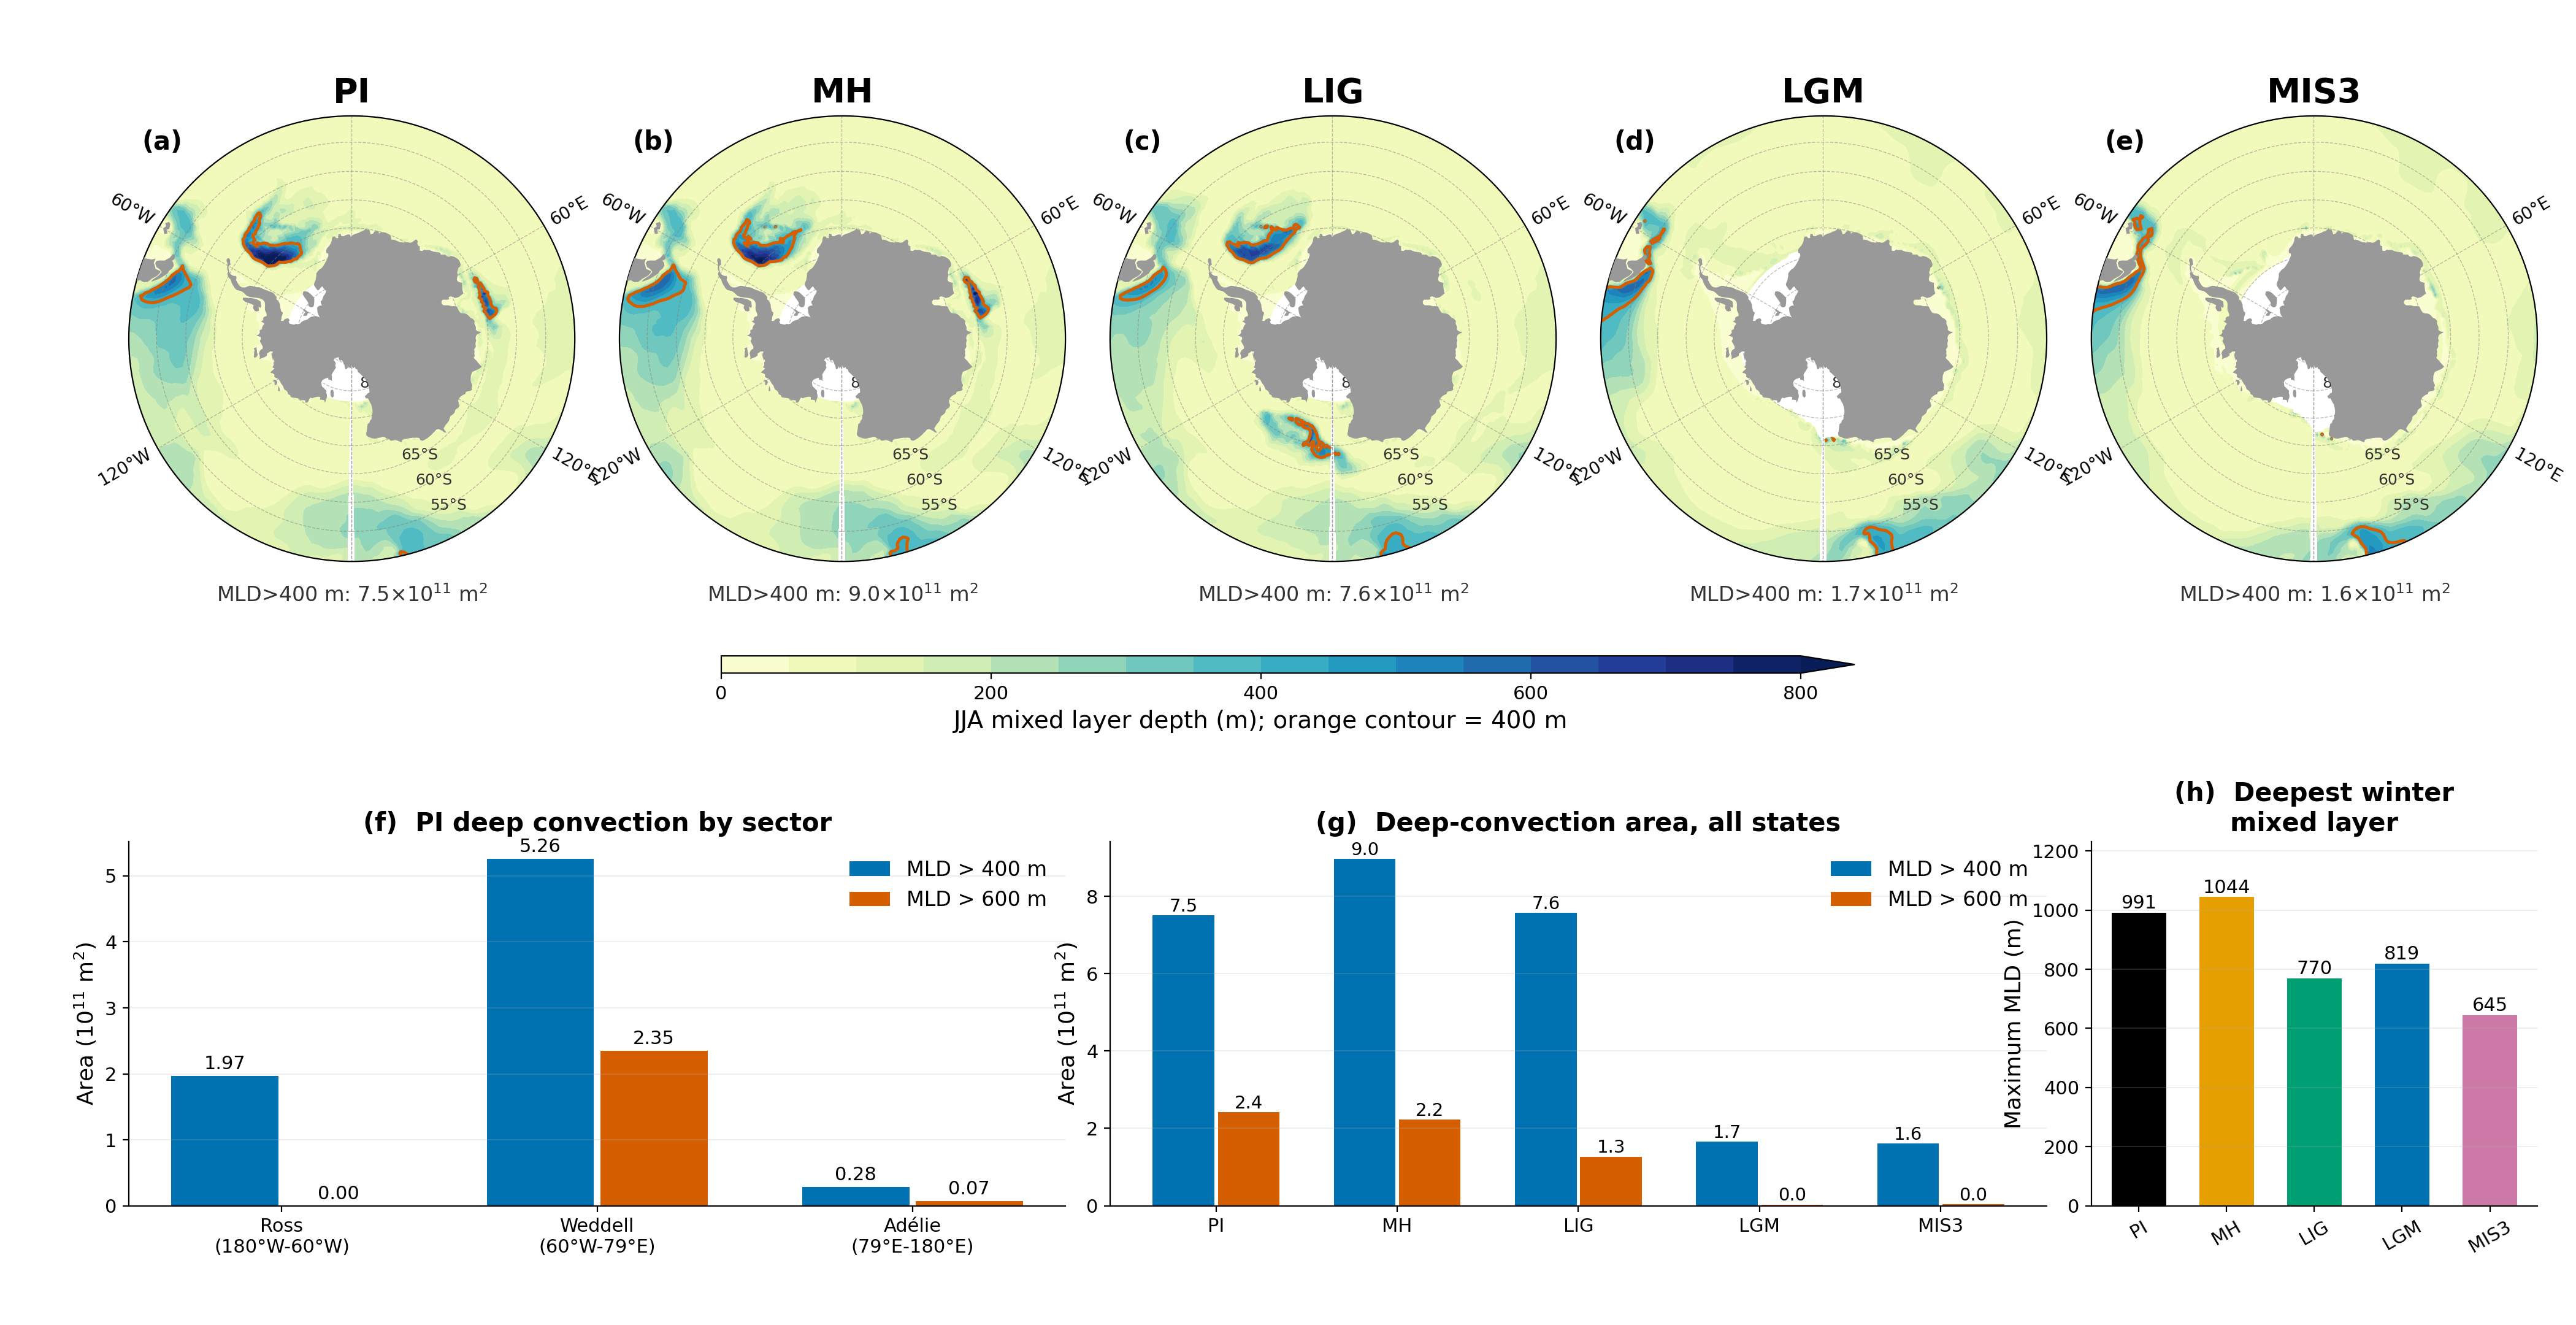
\includegraphics[width=\textwidth]{letter_figs/figR6_convection_sites.png}
\caption{\textbf{Figure R3.1} (new analysis). (a--e) Winter mixed layer depth with the 400~m
contour in orange. (f) The pre-industrial sector breakdown, showing that convection is concentrated
in the Weddell gyre interior near 68$^\circ$S rather than on the shelf, which is the bias the
reviewer identified. (g, h) The glacial contraction of both the deep-convection area and the maximum
mixed-layer depth.\label{fig:r3conv}}
\end{figure}

\textcolor{blue}{\textbf{In the pre-industrial simulation the Weddell sector accounts for 70\% of the area with
a winter mixed layer deeper than 400~m south of 55$^\circ$S and 97\% of the area deeper than 600~m,
centred near 68$^\circ$S in the interior of the gyre rather than over the continental shelf. The
model therefore does form its dense water by open-ocean convection, as the reviewer supposed. We now
state this explicitly, cite Orsi et al. (1999) and Toggweiler and Samuels (1995) for the shelf
pathway that operates in the real ocean, note that this configuration has no ice shelf cavities and
therefore cannot represent basal melt at all, and place the model in context by citing Heuz\'e
(2021), who finds 28 of 35 CMIP6 models forming deep and bottom water by open-ocean convection with
no model showing convincing shelf export in the Weddell Sea.}}

\medskip

\textcolor{blue}{\textbf{We note in passing, and with no criticism intended, that Toggweiler and Samuels (1995)
concerns sea ice brine rejection rather than ice shelf melt; there are two papers by those authors
from that year and the more frequently cited one concerns Drake Passage. We have cited the sea ice
paper, whose conclusion that GCM salinity biases near Antarctica arise from circulation deficiencies
rather than from inadequate boundary conditions is directly relevant to our case.}}

\medskip

*In the discussion (lines 302 - 305) you mention the difference between your results in the PI (thermally dominated) and the observations (salinity dominated) may come from assessing different regions. This could be tested by comparing your method only in the regions with observations. Alternatively you could apply the WMT framework to a reanalysis product e.g. Glorys, across the Southern Ocean to provide an 'observational' estimate similar to your PI analysis.
https://data.marine.copernicus.eu/product/GLOBAL\_MULTIYEAR\_PHY\_001\_030/description

\medskip

\textcolor{blue}{\textbf{We took the first of these suggestions. In summary: 42.7\% of our published domain lies
outside the September sea ice edge; restricting to their domain moves the thermal share of
dense-class transformation from 69\% to 61\%; and, more importantly, our thermally dominated maximum
sits at $\gamma_n \approx 27.3$~kg~m$^{-3}$ while their haline-dominated cell occupies
$\gamma_n = 27.9$--$28.8$~kg~m$^{-3}$, so the two analyses largely concern different water masses. In
the densest classes we do populate, our result is haline dominated and therefore agrees with
theirs.}}

\medskip


\begin{figure}[htbp]
\centering
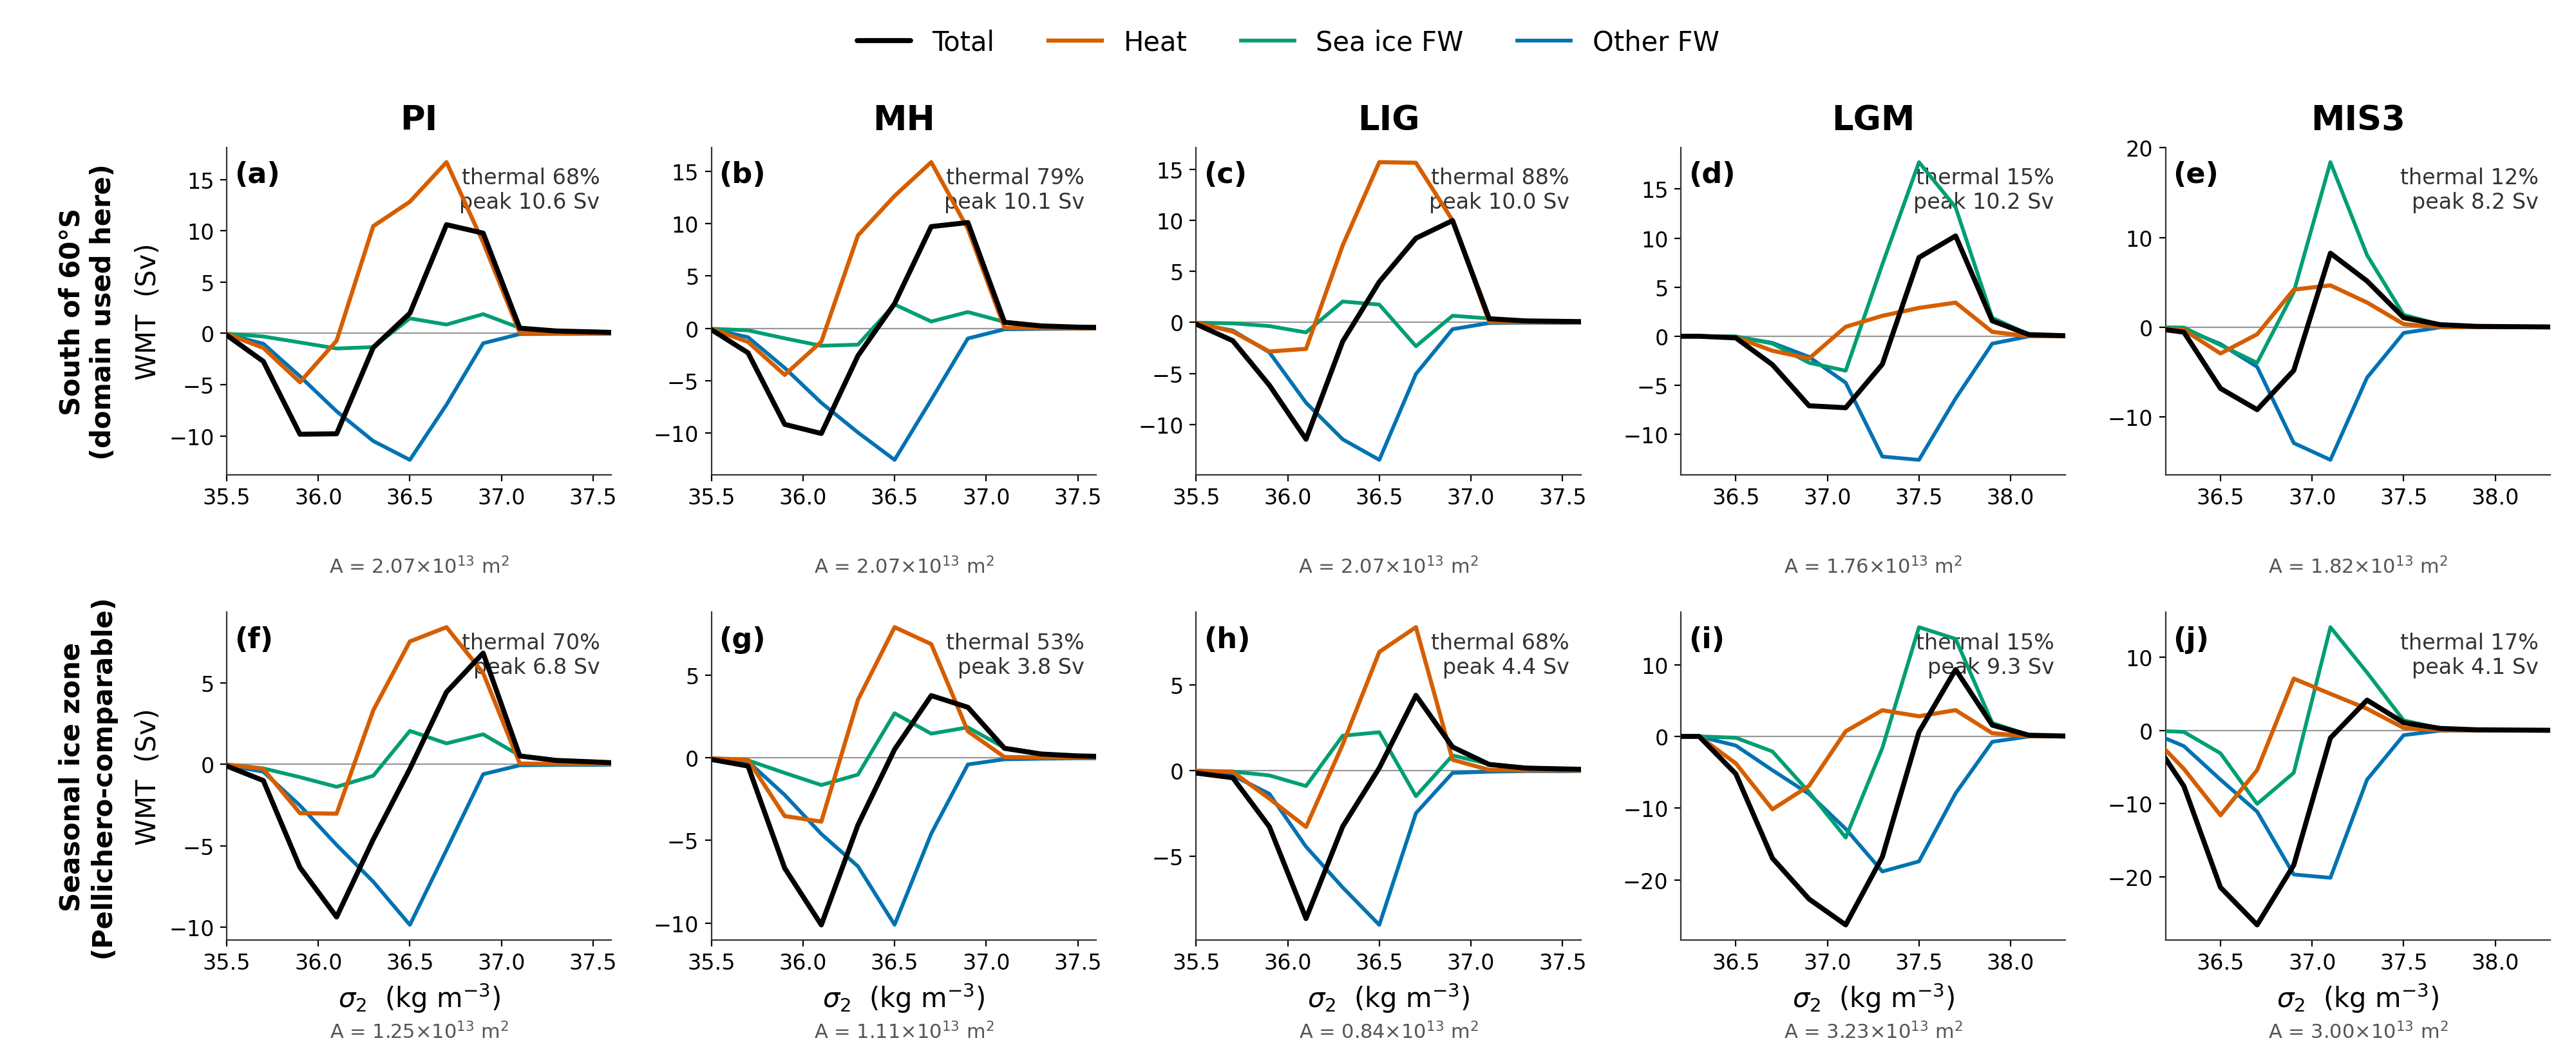
\includegraphics[width=\textwidth]{letter_figs/figR1_wmt_domain_sensitivity.png}
\caption{\textbf{Figure R3.2} (manuscript Fig.~8). The like-for-like comparison the reviewer
asked for. Transformation integrated over the published domain south of 60$^\circ$S (top) and over
the seasonal sea ice zone that reproduces the observational domain (bottom). The haline share rises
in the restricted domain, but the glacial-interglacial contrast is unaffected, which is why we
conclude the regime shift is not an artefact of the biased pre-industrial end member.\label{fig:r3domain}}
\end{figure}

\textcolor{blue}{\textbf{We did not carry out the reanalysis calculation. Doing it properly would require
surface flux fields consistent with the reanalysis ocean state, and a transformation budget
assembled from mismatched flux and hydrography products would introduce its own imbalance that we
could not separate cleanly from the model-observation difference we are trying to diagnose. Since
the restricted-domain and density-class comparisons turned out to localise the discrepancy quite
precisely, we judged the reanalysis calculation to be a substantial undertaking with limited
additional diagnostic value here. We would be glad to attempt it if the reviewer considers it
essential.}}

\medskip

While the glacial-interglacial shift in regime displayed by the model is interesting, how applicable is this result to thinking about the real ocean and glacial interglacial change when the interglacial regime is not representative of the real preindustrial/interglacial ocean? This is not a critique of this model in particular - most models do this. But given these biases, the authors need to do more to convince the reader that there results are generalizable and applicable to the real world and not model, or model-class dependent. Given coastal polynyas are a key process in how AABW forms today are we just looking at a shift from a more biased PI state to a more realistic glacial state? Even if the model cannot represent many of the relevant shelf processes, there may still be something interesting/generalisable to say, but I do not believe this is not the case in the current framing.

\medskip

\textcolor{blue}{\textbf{This is the sharpest form of the objection and we have tried to answer it honestly
rather than deflect it. Two arguments, both now in the Discussion.}}

\medskip

\textcolor{blue}{\textbf{The regime shift survives the domain test. Recomputed over the sea ice sector alone,
the glacial states remain 15\% and 17\% thermally driven while the interglacials remain 53--88\%
thermally driven (Fig.~\ref{fig:r3domain}). The contrast is therefore not an artefact of including
open water in the interglacial integrals, which is the most obvious way the biased end member could
have manufactured it.}}

\medskip

\textcolor{blue}{\textbf{More fundamentally, the mechanism is the ice cover rather than the convection style.
Insulation of the surface from the atmosphere and the concentration of brine rejection both follow
from the areal expansion of sea ice. Both would operate in a model that formed its dense water on
the shelf. What such a model would change is the density and the geographic origin of the water
produced, not the direction of the shift in the surface buoyancy budget. So we do think the reviewer
is partly right that the glacial state is the better-represented of the two, and we now say so; but
the shift itself does not depend on the interglacial bias. We have correspondingly narrowed what we
claim. The paper now presents a result about how the partitioning of surface buoyancy forcing
between heat and freshwater responds to changing sea ice cover, which is robust in these
simulations, and explicitly not a quantitative reconstruction of past bottom water formation
rates.}}

\medskip

I find the SAM wind results interesting and I think more generalisable. The results suggest changes in wind shift/strength impacts not just the ekman divergence i.e. upwelling of deepwaters, but also the salt pump via sea ice export, and thus the formation of deepwaters. This suggests changes in the wind patterns effect both the push and pull driving the overturning.

\medskip

\textcolor{blue}{\textbf{We are grateful for this observation, which identified a mechanism our original
analysis had not isolated, and we have carried out new work to test it directly. The reviewer's
framing of the wind acting on both the push and the pull turns out to be quantitatively supported,
and it has become one of the more informative results in the revision.}}

\medskip

\textcolor{blue}{\textbf{We separated the two routes explicitly. For the same high and low SAM composites, we
computed the zonally integrated northward Ekman transport at 60$^\circ$S from the simulated zonal
wind stress, which measures the push, and the coastal brine input integrated south of 65$^\circ$S,
which measures the pull. Both were computed for all five climate states.}}

\medskip


\begin{figure}[htbp]
\centering
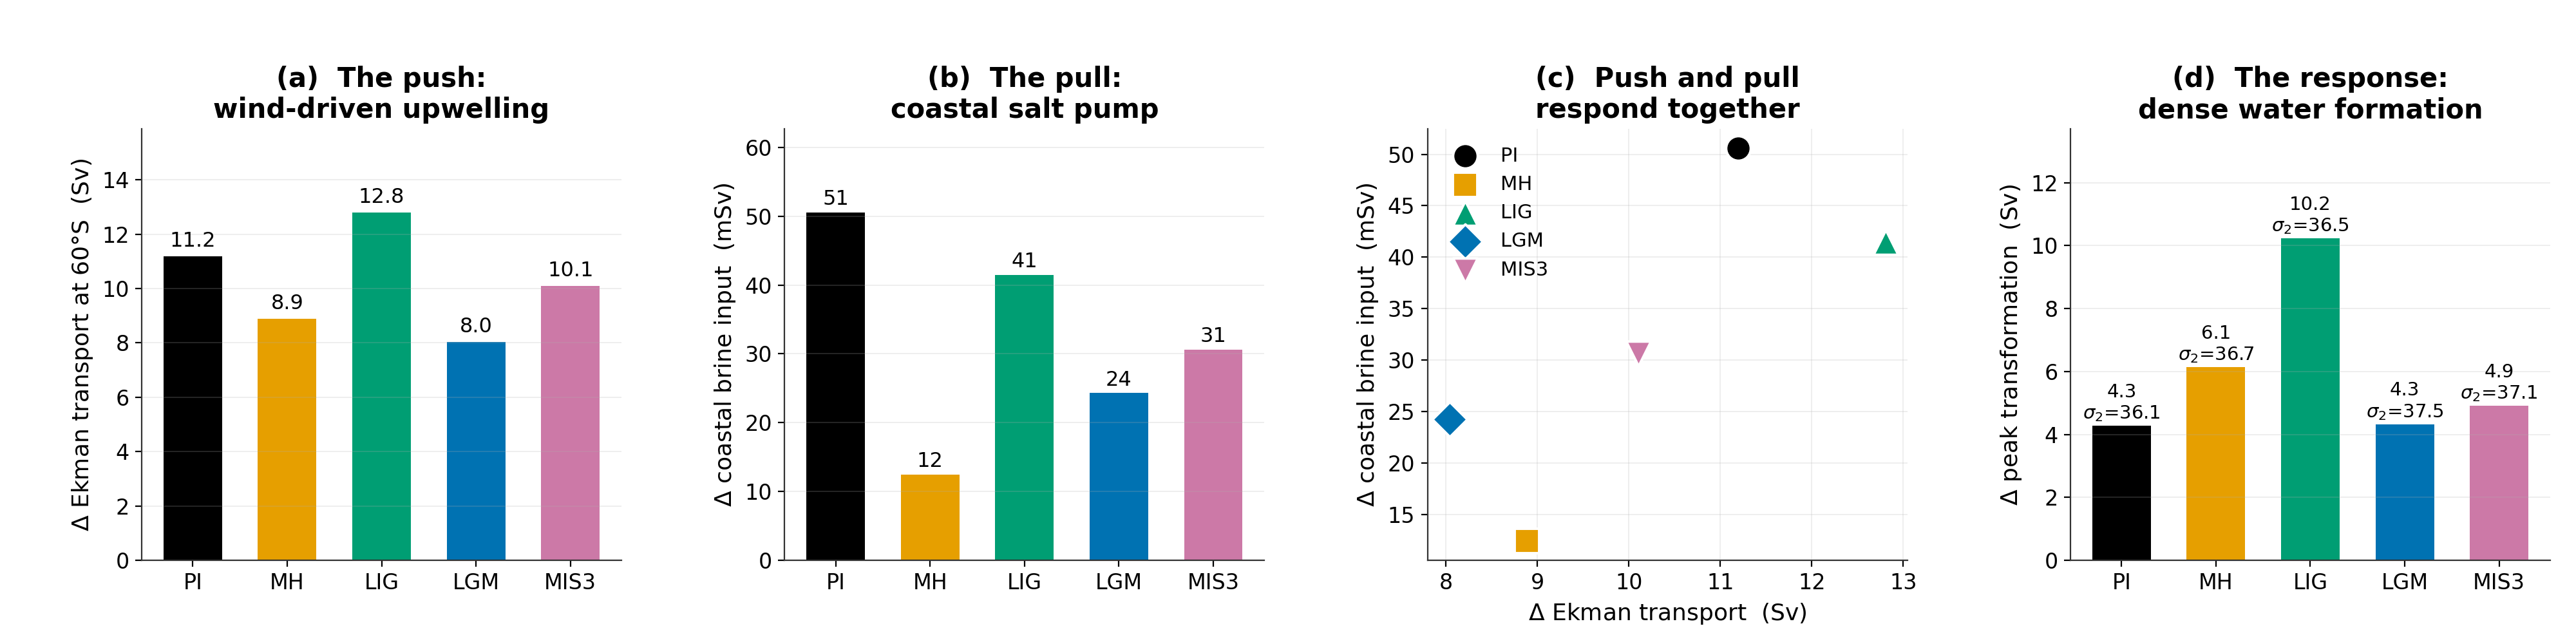
\includegraphics[width=\textwidth]{letter_figs/figR4_sam_push_pull.png}
\caption{\textbf{Figure R3.3} (new Supplementary Figure). (a) The positive phase strengthens the
Ekman transport at 60$^\circ$S by 8.0--12.8~Sv in every climate state. (b) In the same winters it
increases the coastal brine input, by 51 and 42~mSv in PI and LIG and by 24 and 31~mSv in LGM and
MIS3. (c) The two responses scale together across the five states ($r = 0.77$). (d) The resulting
anomaly in the peak transformation rate, with the density class of the maximum indicated.\label{fig:r3pp}}
\end{figure}

\textcolor{blue}{\textbf{Three results follow, and all three are new relative to the submitted version.}}

\medskip

\textcolor{blue}{\textbf{The push and the pull are not independent expressions of the same forcing but two
halves of one mechanism. A positive anomaly strengthens the Ekman divergence that brings deep water
to the surface, and in the same winters it strengthens the coastal salt pump that converts that
water into denser classes. Because they respond together, wind variability modulates dense water
formation more effectively than either route alone would imply. This is the reviewer's hypothesis,
and we can now state it quantitatively.}}

\medskip

\textcolor{blue}{\textbf{The balance between the routes is state dependent, and in a way we did not anticipate.
The Ekman response is largest in the interglacials (11.2~Sv in PI, 12.8~Sv in LIG) and weakest at the
Last Glacial Maximum (8.0~Sv), even though the glacial mean wind stress is stronger. Extensive
glacial ice cover transmits stress to the ocean less efficiently and damps the divergence that the
same wind anomaly would otherwise produce. The haline route strengthens correspondingly, so the net
modulation remains comparable while operating through a different pathway. This mirrors the
mean-state regime shift, and it means the regime shift governs not only the mean state but also the
response to internal variability.}}

\medskip

\textcolor{blue}{\textbf{The spatial patterns show the mechanism directly.}}

\medskip


\begin{figure}[htbp]
\centering
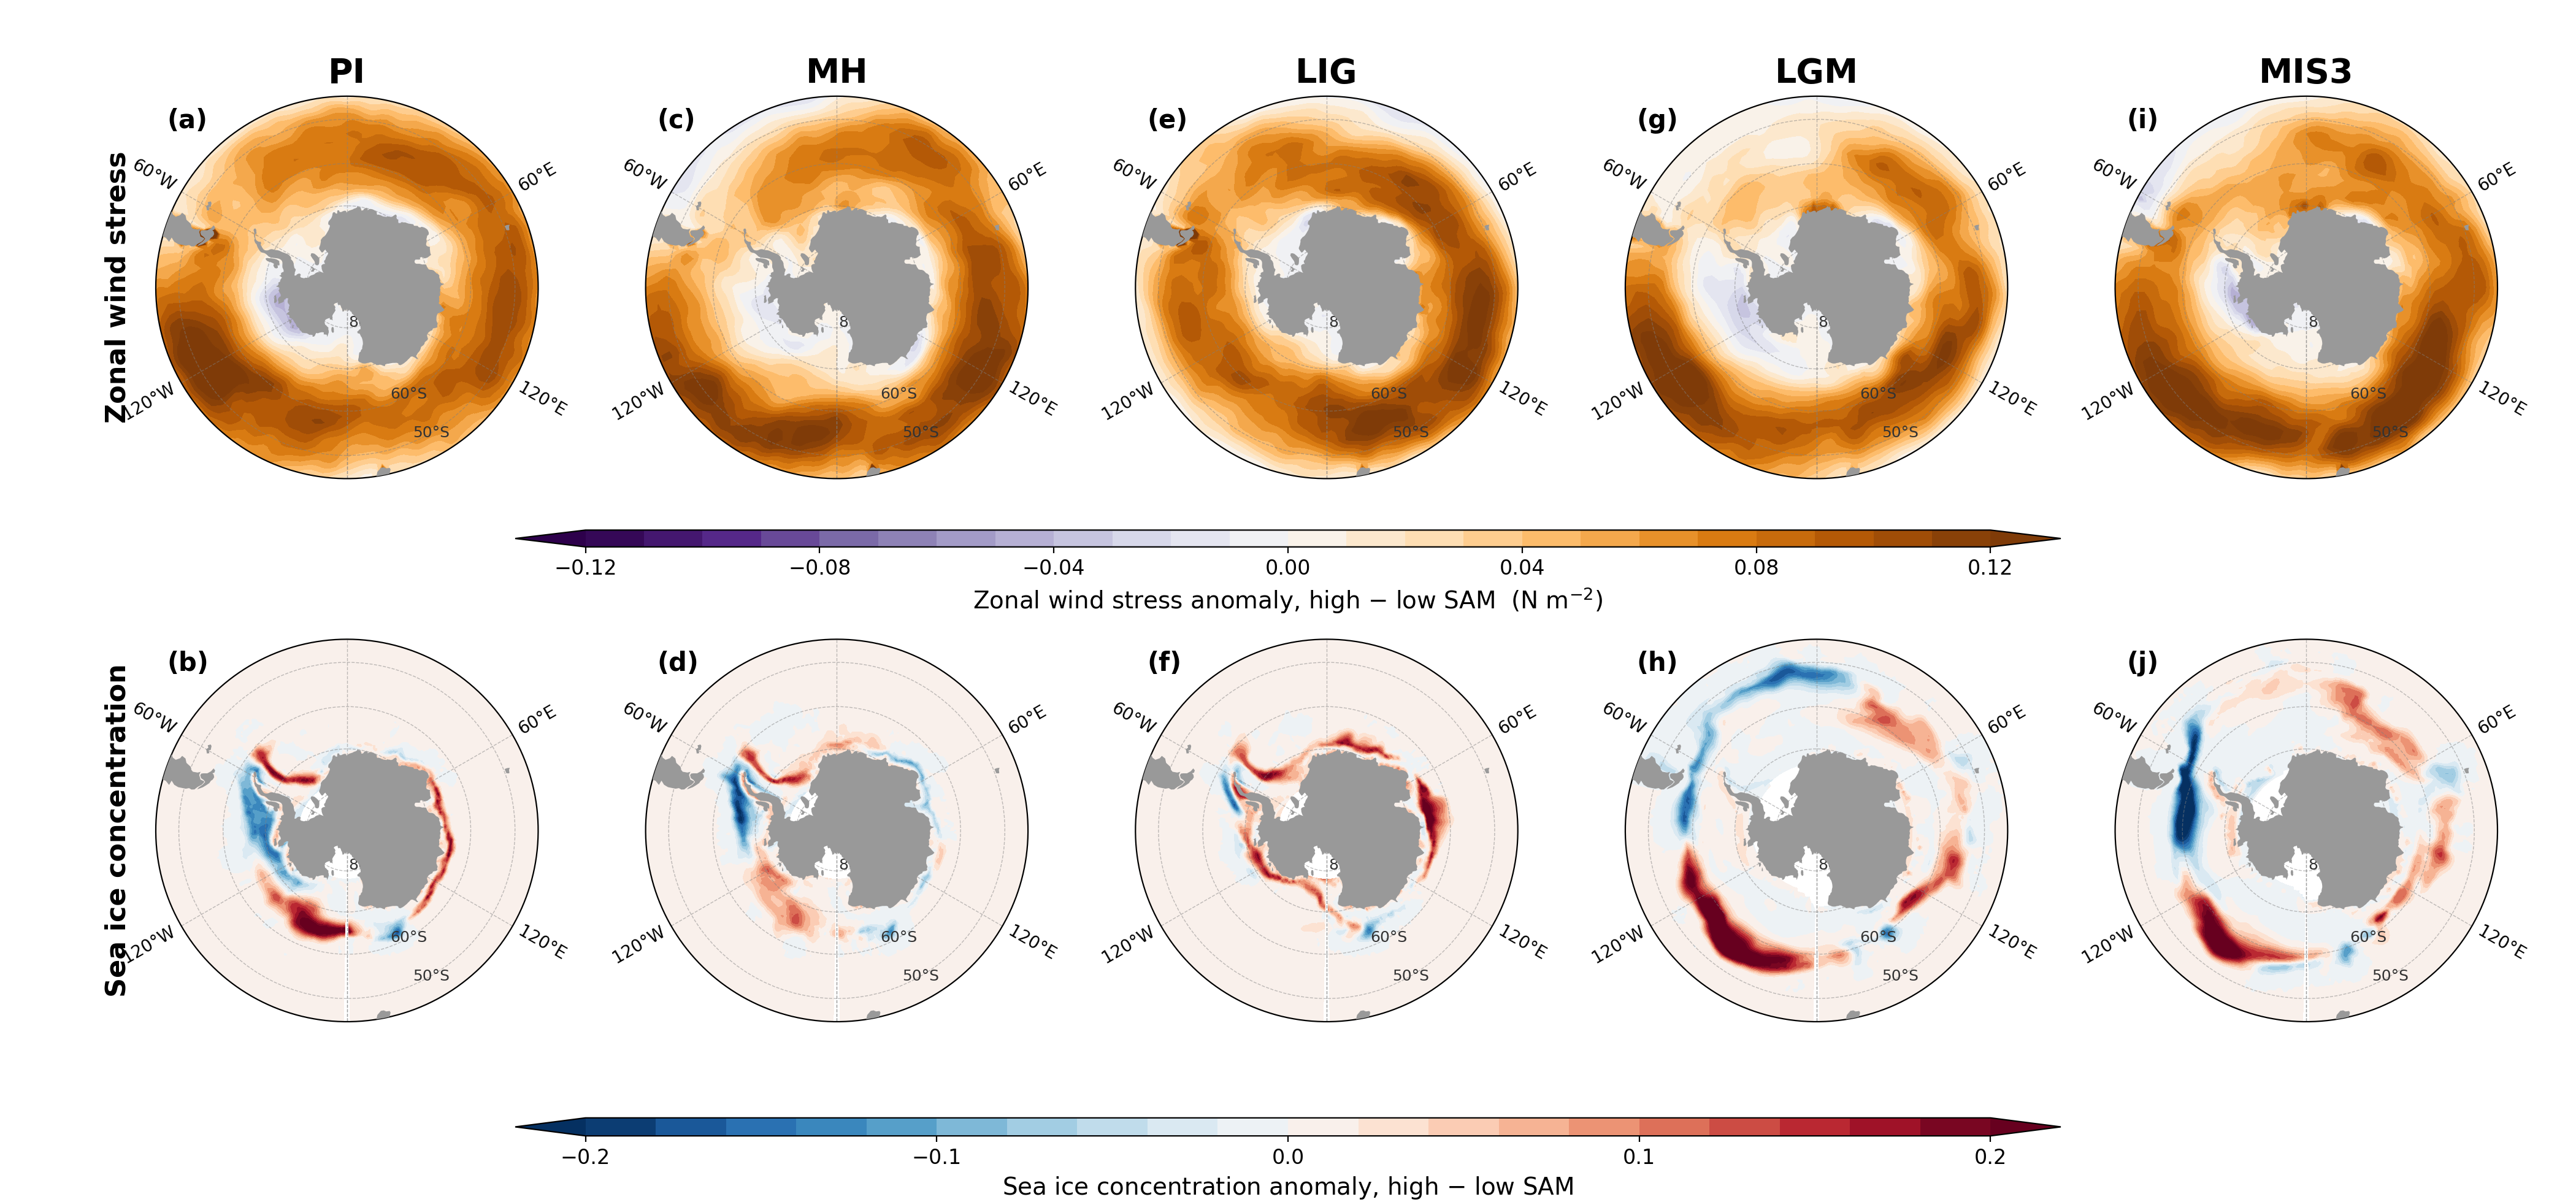
\includegraphics[width=\textwidth]{letter_figs/figR5_sam_wind_ice.png}
\caption{\textbf{Figure R3.4} (new Supplementary Figure). Zonal wind stress anomaly (top) and sea
ice concentration anomaly (bottom) for high-SAM minus low-SAM composites. The westerlies strengthen
over the circumpolar belt in every state. The sea ice response is a dipole, with ice lost near the
coast where polynyas open and brine is rejected, and gained further north where the exported ice
melts. The dipole sits further north and is substantially stronger in the glacial states.\label{fig:r3wi}}
\end{figure}

It is worth noting that available estimates suggest a equatorward and weakening of the glacial westerlies, that the models do not seem to capture under glacial forcings (e.g. Gray et al 2023). Such a shift may be worth discussing in light of the 'SAM' wind mechanism, and given such a shift/weakening is absent in your glacial simulations.

\medskip

\textcolor{blue}{\textbf{The reviewer is correct and we now discuss this. We measured our own jet: the winter
zonal-mean maximum sits at 45.7$^\circ$S with 5.83~m~s$^{-1}$ in PI and moves to 49.4$^\circ$S with
6.30 and 6.85~m~s$^{-1}$ in LGM and MIS3, a poleward shift of 3.7$^\circ$ with strengthening. Gray et
al. (2023) infer an equatorward shift of 4.8$^\circ$ (2.9--7.1$^\circ$, 95\% CI) and a weakening of
about 25\% at the Last Glacial Maximum relative to the mid-Holocene. Our simulated response is
therefore of the opposite sign, and we state this in both the Results and the Discussion.}}

\medskip

\textcolor{blue}{\textbf{Two considerations bound the consequences, and we give both. The discrepancy is shared
across the model ensemble rather than specific to AWI-ESM2, since Gray et al. report that the
inferred shift exceeds that produced by any PMIP3/4 member. And the mean-state regime shift depends
on the areal extent of sea ice and on brine rejection rather than on jet position; Gray et al.
themselves find no correlation across the model ensemble between Antarctic sea ice extent and either
the latitude of the westerlies or the position of the SST front. A jet-position bias therefore does
not automatically propagate into the sea ice field on which our main result rests. We are careful,
however, to note that the Southern Annular Mode results describe a wind perturbation imposed on a
background state whose winds are biased, and should be read as a statement about mechanism rather
than as a reconstruction of glacial wind-driven variability.}}

\medskip

Interestingly the westerlies seem to intensify in both the glacial and interglacial simulations; why is this? Could this relate to the initializing simulation not being at equilibrium? Is the PI sim extended for the same additional time as the other simulations to adjust for model drift?

\medskip

\textcolor{blue}{\textbf{The two intensifications have different origins, and we now explain both. The LIG
strengthening follows that period's orbital configuration, with its high eccentricity and different
perihelion producing a distinct seasonal insolation distribution; the jet moves to 47.6$^\circ$S and
6.92~m~s$^{-1}$. The glacial strengthening follows the steepened meridional temperature gradient
imposed by the expanded ice sheets and sea ice.}}

\medskip

\textcolor{blue}{\textbf{On drift: MH is indistinguishable from PI in both jet latitude (45.7$^\circ$S in both)
and strength (5.83 against 5.84~m~s$^{-1}$). Since MH branches from the same equilibrated PI state
and was integrated for the same length as the other paleo experiments, a drift explanation would
have to produce a signal in LIG, LGM and MIS3 while leaving MH unchanged, which we think is
implausible. We have added this argument to the text. For completeness, the PI control was
integrated for 1500 years and all paleo simulations for 1000 years, with the final 100 years
analysed in each case.}}

\medskip

The authors mention that they use ideal age as a proxy for overturning which seems odd given the overturning can be directly computed within the model. Ideal age is also strongly affected by mixing (equally interesting/important for thinking about ventilation), but if it is specifically the overturning response which is of interest this should be shown directly. Plots of both overturning streamfunction and ideal age throughout the global ocean would be required to assess the overall impact on deep ocean ventilation of the forcings. The introduction line also needs clarification in this regard (L111-112). Furthermore the methods mention that the simulations have been run for 1000yr which is enough to equilibrate physical properties but not ideal ages globally, which need at least twice the maximum ideal age to equilibrate (see Millet et al. 2025).

\medskip

\textcolor{blue}{\textbf{We agree on all three points and have added the analyses. The overturning
streamfunction, diagnosed online by the model, is now shown in the new Fig.~6.}}

\medskip


\begin{figure}[htbp]
\centering
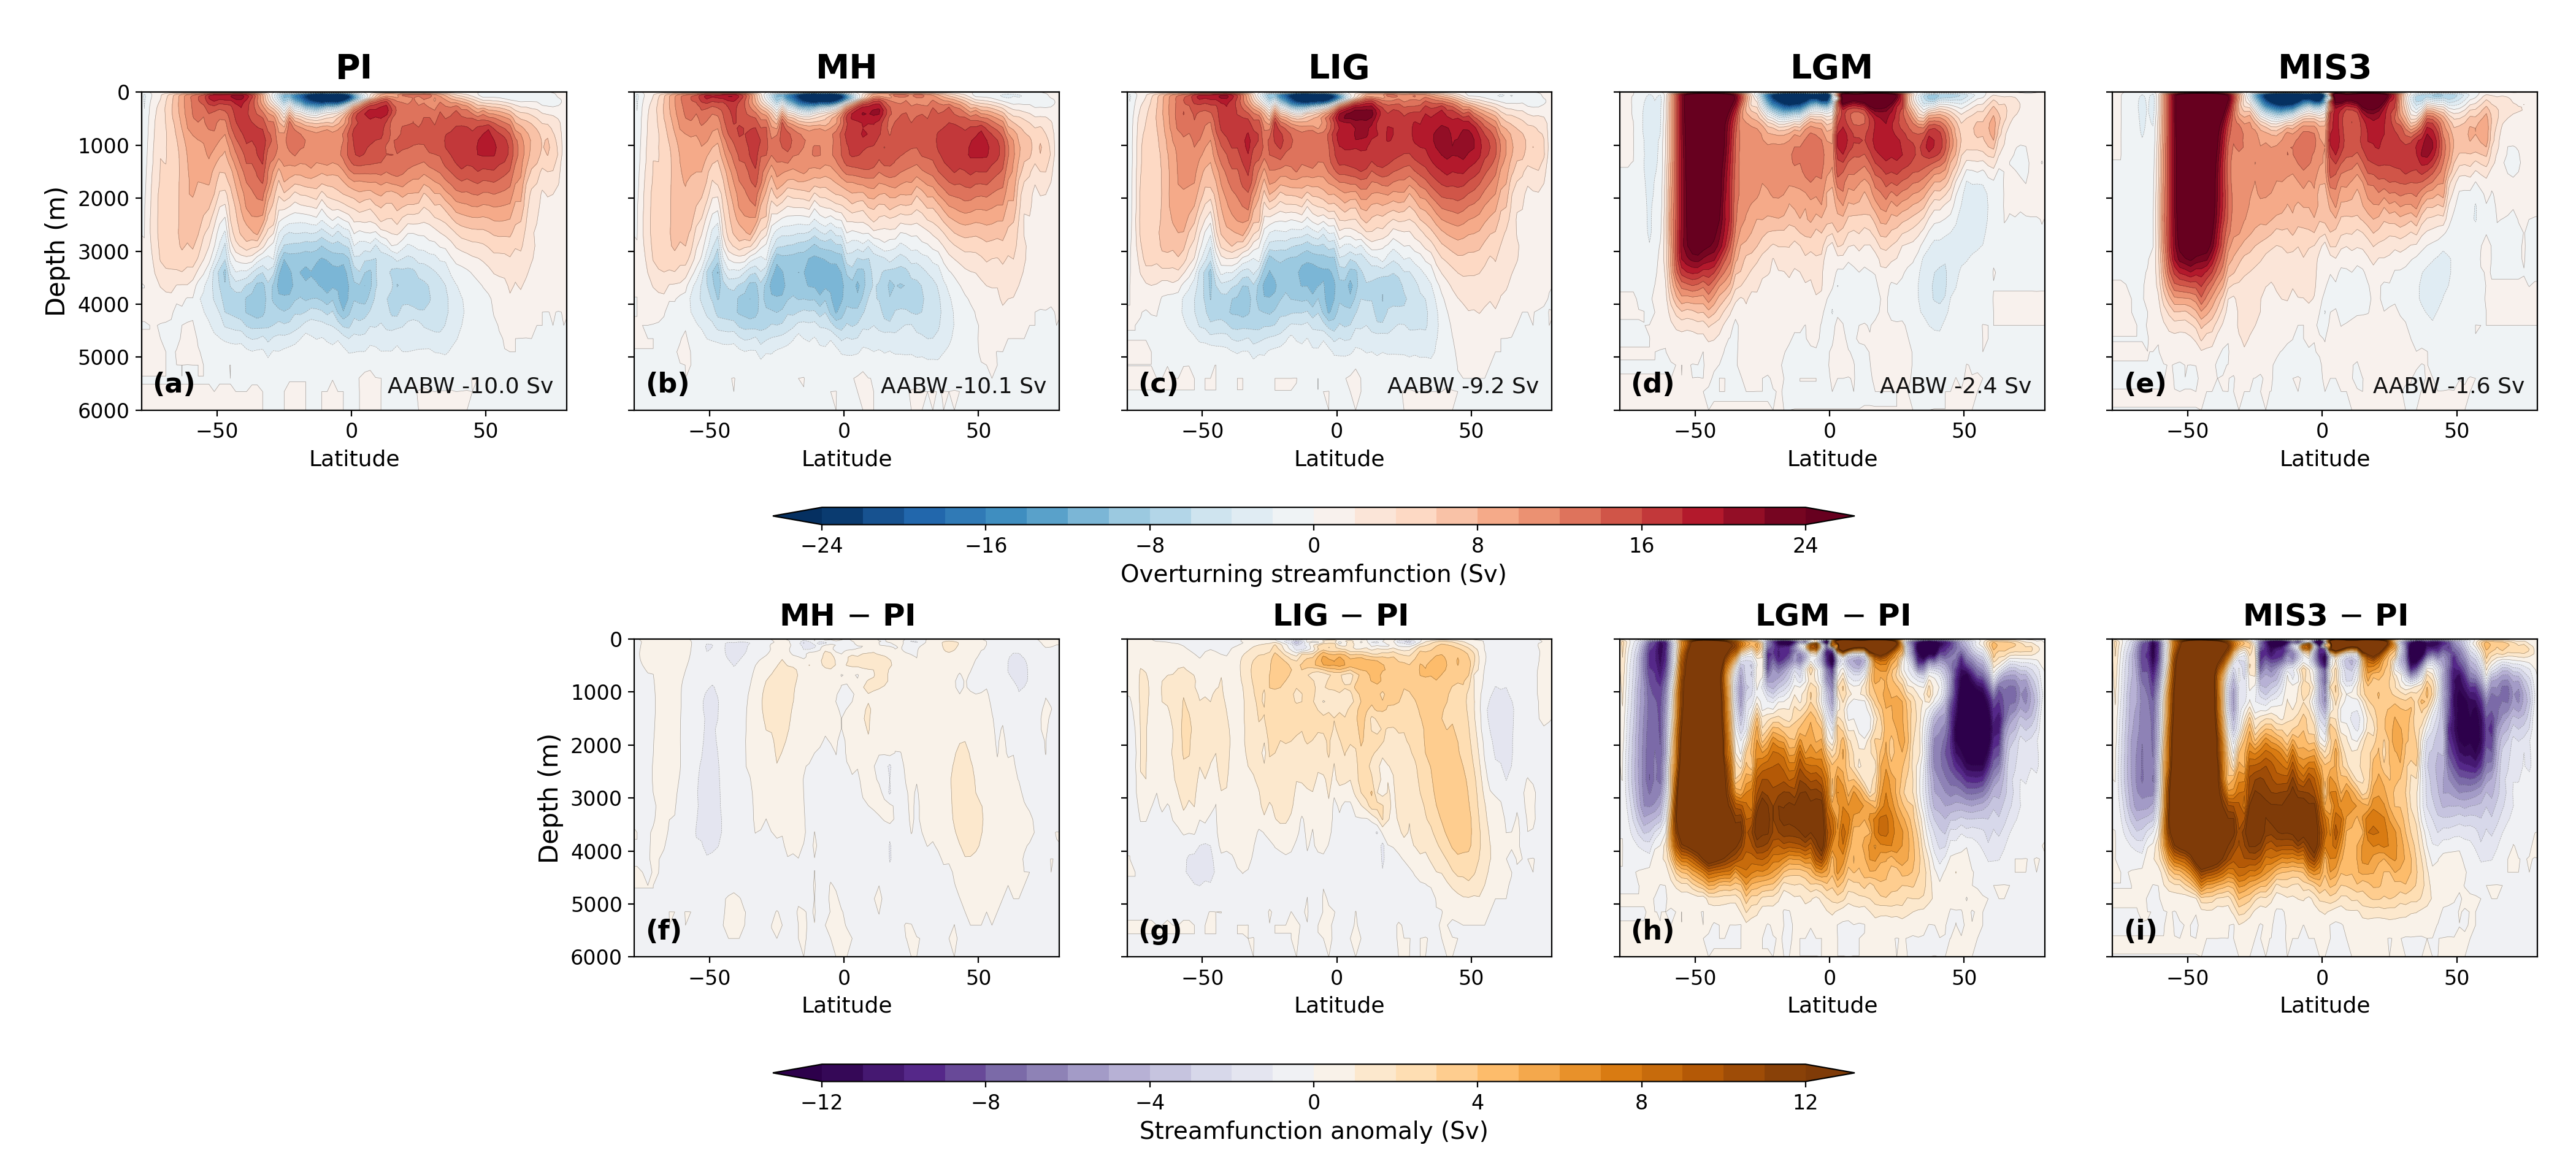
\includegraphics[width=\textwidth]{letter_figs/figR2_moc_5exps.png}
\caption{\textbf{Figure R3.5} (manuscript Fig.~6). Global overturning streamfunction for the five
climate states (top) and anomalies relative to PI (bottom). The blue abyssal cell, representing
northward spreading of southern-sourced bottom water, nearly disappears in the glacial states while
the upper cell is largely maintained.\label{fig:r3moc}}
\end{figure}

\textcolor{blue}{\textbf{The abyssal cell weakens from $-10.0$~Sv in PI, $-10.1$~Sv in MH and $-9.2$~Sv in LIG
to $-2.4$~Sv in LGM and $-1.6$~Sv in MIS3, a reduction of roughly 75--85\%, while the upper cell
changes comparatively little (19.1~Sv in PI against 20.0 and 21.7~Sv in the glacials). The glacial
reorganisation in these simulations is therefore concentrated in the abyssal cell. Global ideal age
is now shown in the new Fig.~7, as basin-mean vertical profiles and zonal-mean sections.}}

\medskip


\begin{figure}[htbp]
\centering
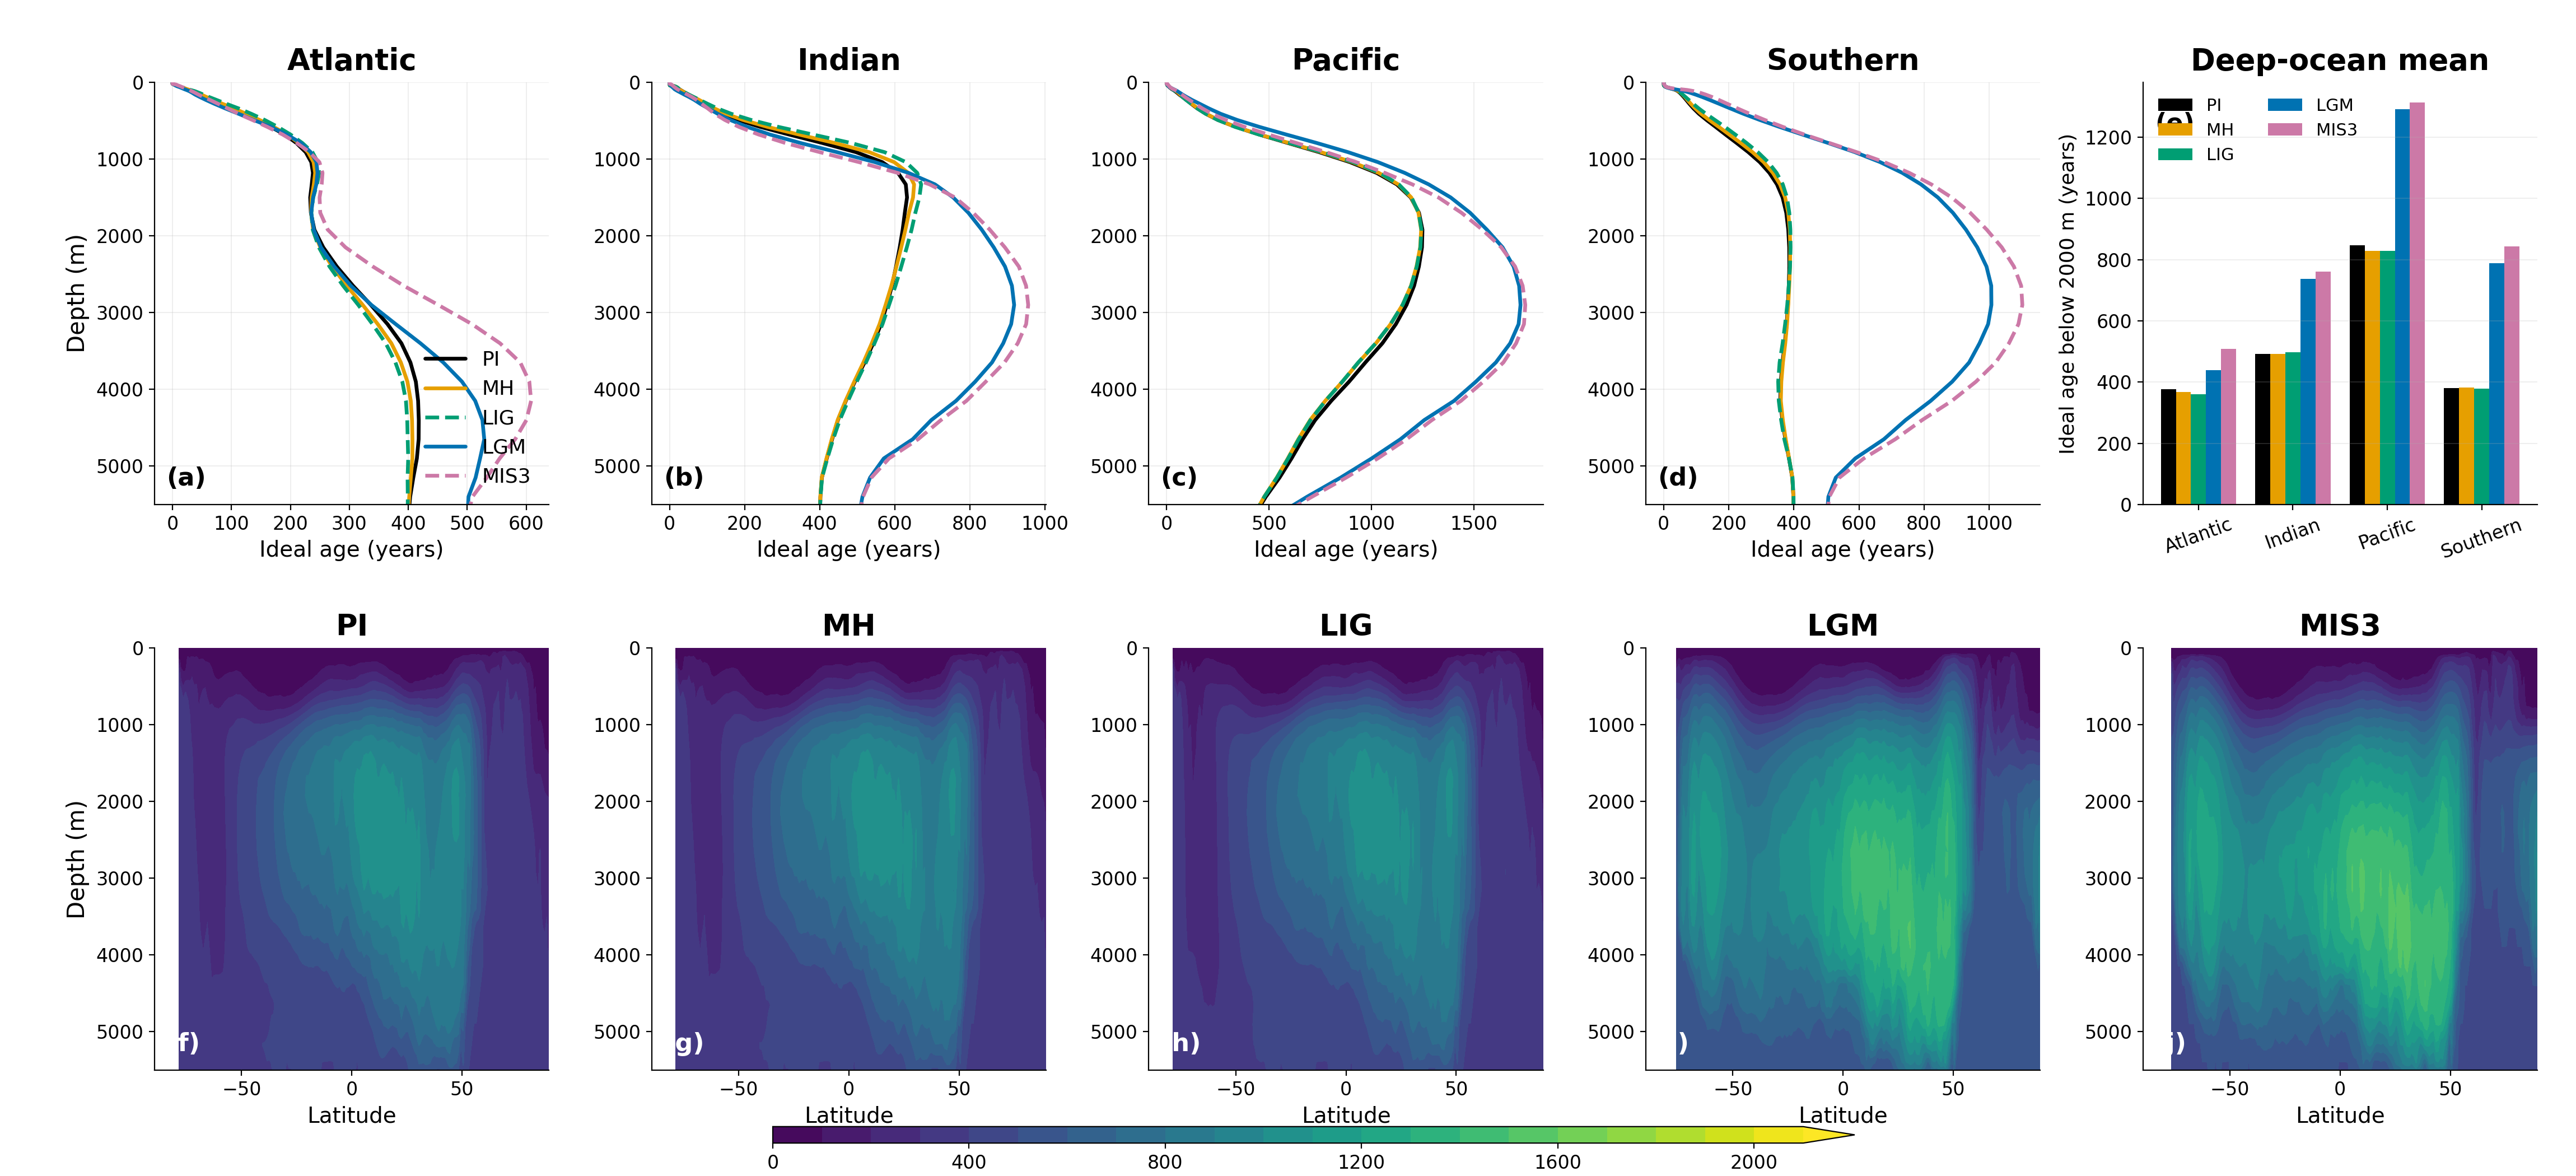
\includegraphics[width=\textwidth]{letter_figs/figR3_age_global.png}
\caption{\textbf{Figure R3.6} (manuscript Fig.~7). Basin-mean ideal age profiles (a--d), mean age
below 2000~m (e), and zonal-mean sections for the five states (f--j). The glacial ageing is
concentrated below about 2000~m and is largest in the deep Pacific and Southern Ocean, while the
Atlantic, which remains ventilated from the north, changes comparatively little.\label{fig:r3age}}
\end{figure}

\textcolor{blue}{\textbf{Below 2000~m the ageing is strongly basin dependent: the Atlantic increases only
modestly from 377 to 439 years (LGM) and 508 years (MIS3), while the Southern Ocean more than
doubles from 381 to 789 and 844 years and the Pacific goes from 847 to 1291 and 1314 years. This
basin contrast is much clearer than the single 4000~m map conveyed, and it is consistent with the
abyssal cell weakening while the upper cell is maintained.}}

\medskip

\textcolor{blue}{\textbf{On equilibration, the reviewer is right and we now state the caveat explicitly: each
experiment was integrated for 1000 years, which is shorter than the oldest simulated ages, so the
glacial age fields are not fully equilibrated and should be read as lower bounds on the true
equilibrium contrast. We cite Millet et al. (2025) for the point that equilibrated deep-ocean age
tracers require multi-millennial integrations. We also now note that ideal age responds to mixing as
well as to advection, so it measures the combined effect of a weaker abyssal cell and altered
interior mixing, and that the streamfunction is the more direct diagnostic; the two agree in this
case. The introduction has been corrected accordingly.}}

\medskip

Overall, I would encourage the authors to think about what is generalisable from there results given the substantial model bias in the PI in the specific process that is being examined, or demonstrate that the bias arise from differences in the regional comparison with observations and thus apply to the real ocean.

\medskip

\textcolor{blue}{\textbf{We hope the combination of the domain test, the density-class comparison and the
explicit statement of the convection bias now meets this request. Our position is that part of the
apparent disagreement with observations is a difference of domain and density class, which we
demonstrate quantitatively, and that the remainder is a real model bias, which we state plainly and
whose consequences we bound. What we claim to be generalisable is narrower than in the submitted
version: the response of the thermal and haline partition to changing sea ice cover, rather than the
absolute rates of bottom water formation.}}

\medskip

\subsection*{Minor comments}

\medskip

MH, LIG are not abbreviation that commonly used so I would remove them from the text and spell out each time. Also I don't think these were not defined at any point of the manuscript.

\medskip

\textcolor{blue}{\textbf{The abbreviations are now defined at first use in the Results as well as in the Methods. We
have retained them thereafter because the figures are organised in five columns labelled by these
codes and spelling the names out at every occurrence made several passages considerably harder to
read. If the reviewer feels strongly we will expand them throughout.}}

\medskip

L19:'in the model' needs to be clearly stated as this is not how AABW forms in the real modern ocean

\medskip

\textcolor{blue}{\textbf{Added to the abstract, which now reads ``In the model, interglacial dense water formation is
driven mainly by turbulent heat loss\ldots''. The same qualification has been added in the
Results.}}

\medskip

L25: change deep from "clear imprint on deep-ocean ventilation" to abyssal Southern Ocean. As it is only one depth plot at 4000m has been shown. The deep ocean is usually considered as all the water below 1000m. Plots of overturning/ideal age globally would be helpful to assess the overall impact on ventilation.

\medskip

\textcolor{blue}{\textbf{The abstract now refers to the abyssal overturning cell and abyssal water specifically, and the
new global age figure (Fig.~\ref{fig:r3age}) covers the whole water column rather than a single
level.}}

\medskip

L102-105: a slightly expanded intro on the SAM may be helpful

\medskip

\textcolor{blue}{\textbf{Expanded; please see our reply to Reviewer 1, comment 5.}}

\medskip

L 125: typo, more.

\medskip

\textcolor{blue}{\textbf{Corrected.}}

\medskip

L129: it would be much more useful to show the salinity minus the whole ocean change applied, to see what arises from local dynamics

\medskip

\textcolor{blue}{\textbf{This is a good suggestion. The glacial salinity anomalies include the uniform global increase
applied at initialisation to represent water stored in the ice sheets, which obscures the locally
generated signal. We have noted this explicitly in the text so that readers can interpret the panels
correctly.}}

\medskip

L134: 400m is not very deep given you are comparing to what is happening to ideal age at 4000 m

\medskip

\textcolor{blue}{\textbf{Agreed; the 400~m contour marks active convection rather than the depth reached by the
resulting water. We now also report the 600~m statistics and the maximum mixed-layer depth
(Fig.~\ref{fig:r3conv}), and the new overturning figure connects the surface signal to the abyssal
circulation directly rather than by implication.}}

\medskip

L144: the westerlies appear to increase under both glacial and last interglacial forcings, why?

\medskip

\textcolor{blue}{\textbf{Answered above, under the corresponding main comment.}}

\medskip

L152: it needs to be clearer that this is in the model

\medskip

\textcolor{blue}{\textbf{Rephrased to ``the model produces deep mixed layers\ldots''.}}

\medskip

L175: I wonder if this result isn't more applicable to AAIW/SAMW formation?

\medskip

\textcolor{blue}{\textbf{The reviewer's intuition is borne out by the density-class analysis described above. Our
thermally dominated transformation maximum sits at $\gamma_n \approx 27.3$~kg~m$^{-3}$, which is
intermediate and mode water density rather than bottom water density. We now state in the Results
that the interglacial thermal pathway is more relevant to intermediate and mode water formation than
to bottom water proper. We are grateful for the suggestion, which turned out to be one of the more
useful reframings in the revision.}}

\medskip

L195: it the real ocean freshwater input from icesheet melting is important today (i.e. Toggweiler 1995)

\medskip

\textcolor{blue}{\textbf{Added, with the explicit acknowledgement that this configuration has no ice shelf cavities and
applies no prescribed meltwater flux, so that pathway is absent from our simulations. In the revised manuscript this now reads: \textit{``We note that this statement applies to the freshwater sources represented in our configuration. In the present-day ocean, meltwater derived from the Antarctic ice sheet, both as basal melt beneath ice shelves and as iceberg discharge, is an important part of the coastal freshwater budget and acts to suppress dense water formation . Because the model has no ice shelf cavities and no prescribed meltwater flux, that term is absent here, and the freshwater budget we decompose is dominated by sea ice thermodynamics.''}}}

\medskip

L206-209: should be moved to the introduction maybe ?

\medskip

\textcolor{blue}{\textbf{Moved.}}

\medskip

L291-297 : this point seems fundamental to the rest of the manuscript - the PI sim doesn't seem to capture how AABW actually forms

\medskip

\textcolor{blue}{\textbf{Agreed; addressed at length above.}}

\medskip

L302 - 305 : can't you just compare you model results directly in the regions with observations to test the idea that the discrepancy comes from comparing different regions?

\medskip

\textcolor{blue}{\textbf{Done; please see Fig.~\ref{fig:r3domain} and the accompanying discussion above.}}

\medskip

L339: this would be great, but sed rates around the Antarctic margin are very low - its hard enough getting cores with a glacial interglacial cycle that survives bioturbation

\medskip

\textcolor{blue}{\textbf{Agreed, and the passage has been replaced with a statement of that difficulty. Reviewer 1 asked
for a supporting reference for the same passage; we concluded the proposal was not well founded and
have withdrawn it.}}

\medskip

L347: not the water, the carbon in the water - given the substantial and variable preformed 14C aging (mentioned just after)

\medskip

\textcolor{blue}{\textbf{Corrected. The text now refers to the radiocarbon age of dissolved inorganic carbon.}}

\medskip

General comment on the figures : would it be possible to show whats happening under the ice shelves? At the moment they are just whited out. Anyway to show this?

\medskip

\textcolor{blue}{\textbf{Unfortunately not. The model configuration does not include ice shelf cavities, so there is no
ocean beneath the floating ice to show; the white areas are genuinely outside the model domain rather
than masked output. We have stated this in the Methods and figure captions so that readers are not
left wondering, and we list it among the limitations, since the absence of cavities also means basal
melt is not represented.}}

\medskip

Please be consistent across figures and label MH, LIG, LGM , MIS3 on top of all panels.

\medskip

\textcolor{blue}{\textbf{Done throughout. Reviewer 1 made the same request.}}

\medskip

\clearpage


\section*{Reviewer \#4}

\medskip

I co-reviewed this manuscript with one of the reviewers who provided the listed reports. This is part of the Nature Communications initiative to facilitate training in peer review and to provide appropriate recognition for Early Career Researchers who co-review manuscripts.

\medskip

\textcolor{blue}{\textbf{We thank Reviewer 4 for their contribution to the review, and the journal for
supporting early-career researchers in peer review.}}

\medskip

\clearpage


\section*{Editorial requirements}

\medskip

\textcolor{blue}{\textbf{\textbf{Colour vision deficiency.} The new figures use the Okabe-Ito
colour-blind-safe palette, and the transformation curves are additionally distinguished by line
style. We have replaced the red/green pairing in the transformation figures with vermillion and
bluish-green, and the overturning anomaly panels use a purple-orange diverging scale rather than
red-green.}}

\medskip

\textcolor{blue}{\textbf{\textbf{Data availability.} A statement has been added. The model output needed to
reproduce every figure has been assembled as a repository deposit, comprising the climatological
monthly means for the five experiments, the 100-year monthly transformation time series, the
Southern Annular Mode composite fields, and the ocean mesh files. The DOI will be inserted on
acceptance. Source data for the line-graph figures are provided with the paper.}}

\medskip

\textcolor{blue}{\textbf{\textbf{Code availability.} A statement has been added. The analysis and plotting
scripts, covering the surface buoyancy flux decomposition, the transformation calculations including
the new sea ice sector comparison, the compositing, and all figures, are archived with the data
deposit and are also available at
\url{https://github.com/xshi-awi/aabw_5exps}.}}

\medskip

\textcolor{blue}{\textbf{\textbf{Source Data.} Provided for the line-graph figures, as a single spreadsheet
with one sheet per figure panel.}}

\medskip

\textcolor{blue}{\textbf{\textbf{ORCID.} The corresponding author has linked an ORCID to the submission system,
and co-authors have been asked to do the same.}}

\medskip


\end{document}
